%!TEX program = lualatex
%!TEX encoding = UTF-8 Unicode  
%!TEX root = chapter02.tex  
\documentclass[main.tex]{subfiles} 
\begin{document} 
%----------------------------------------------------------------------------------------
%	CHAPTER 2
%----------------------------------------------------------------------------------------
\cleardoublepage 
\loadgeometry{marginlayout}  
\pagestyle{scrheadings} % Print headers again  
\KOMAoptions{
	headwidth=textwithmarginpar,
	headsepline=true,
	headsepline= 0.5pt,
	footwidth=textwithmarginpar,
}   
\onehalfspacing 
\setcounter{chapter}{1}
\chapter{Probabilité conditionnelles et indépendance}
%\margintoc
\section{Lois de probabilités (vu en 2nde)}
Une \textbf{expérience aléatoire}  est une expérience \textbf{renouvelable à l'identique}, dont on connait les \textbf{issues}, et dont le résultat est \textbf{imprévisible}.\\
Chaque renouvellement de l'expérience s'appelle \textbf{épreuve}.
\begin{description}
	\item[$\bullet$ une issue] est notée  $\omega$, ou $\omega_1$, $\omega_2, \ldots$. à lire \og oméga \fg{}
	\item[$\bullet$ l'univers $\Omega$] désigne l'ensemble des issues possibles  $\Omega=\{ \omega_1; \omega_2; \omega_3;\ldots ;\omega_n\}$. \\
	$n$ désigne le nombre total d'issues.
	\item[$\bullet$ un événement $E$] est une partie de $\Omega$ : $E\subset \Omega$
	\item[$\bullet$  $\omega$ \textbf{réalise} l'événement $E$]  signifie $\omega\in E$. 
\end{description} 
\begin{definition}[définition constructive d'une loi de probabilité] Pour un univers $\Omega=\{ \omega_1, \omega_2, \ldots , \omega_n\}$.
	\begin{enumerate}[label=\alph*),leftmargin=*]
		\item on attribue à chaque événement élémentaire $\omega$ une probabilité positive $p(\omega)\geqslant 0$
		\marginnote{
			\begin{tBox}[leftline=false]\centering
				$P(\Omega)=\sum_{\omega\in\Omega} p(\omega)=1$
			\end{tBox}
		} 
		\item la somme des probabilités des événements élémentaires est égale à $1$ :
		
		$
		p(\omega_1)+p(\omega_2) +\ldots+p(\omega_n)=1
		$ 
		\marginnote{
			\begin{tBox}[leftline=false]\centering
				$P(\{\omega\}) =p(\omega)$
				
				$P(E)=\sum_{\omega \in E} p(\omega)$
			\end{tBox}
		}     
		\item Pour tout événement $E$, la probabilité $P(E)$ est égale à la probabilité des événements élémentaires qui le composent.
		
	\end{enumerate}	 
\end{definition}  
\textbf{Convention lycée} Dans tout exercice où figurent des expressions tel que \og dés équilibrés \fg{}, \og tirage au hasard \fg{}, \og urnes opaque et jetons indiscernables au toucher \fg{}... le modèle choisi sera celui de l’équiprobabilité : tous les événements élémentaires ont la même probabilité.

\begin{definition}[situation d'équiprobabilité] Pour un univers $\Omega=\{ \omega_1, \omega_2, \ldots , \omega_n\}$.
	\marginnote{
		\begin{tBox}[leftline=false] Le  $\operatorname{Card}(E)$  (lire \textbf{cardinal}) est le nombre d'issues qui réalisent $E$.
		\end{tBox}
	} 
	\begin{enumerate}[label=\alph*),leftmargin=*] 
		\item   
		$
		p(\omega_1)=p(\omega_2) =\ldots=p(\omega_n)=\frac{1}{\operatorname{Card}(\Omega)}
		$      
		\item Pour tout événement $E$ on a $P(E)=\frac{\operatorname{Card}(E)}{\operatorname{Card}(\Omega)}$.
	\end{enumerate}	 
\end{definition}
\begin{theorem}[formulaire]
	Toute loi de probabilité sur un univers $\Omega$ vérifie les propriétés suivantes :
	\marginnote{
		\begin{tBox}[leftline=false]\centering loi unitaire
		\end{tBox}
	} 
	\begin{enumerate}[label={\textbf{(P\arabic*)}},leftmargin=*]
		\item $P(\Omega)=1$ et $P(\emptyset)=0$
		\marginnote{
			\begin{tBox}[leftline=false]\centering loi positive
			\end{tBox}
		} 
		\item Pour tout événement $A$ \hfill  $0\leqslant P(A)\leqslant 1$ 
		\item \marginnote{
			\begin{tBox}[leftline=false]\centering $P(A)+P(\overline{A})=1$
			\end{tBox}
		}  Pour tout événement $A$  \hfill    $$P(\overline{A})=1-P(A)$$  
		\marginnote{
			\begin{tBox}[leftline=false]\centering loi additive
			\end{tBox}
		} 
		\item  Si $A$ et $B$ sont des événements incompatibles  alors :
		$$\text{Si $A\cap B=\emptyset$ alors } P(A\cup B)=P(A)+P(B)$$
		\item  Pour tous événements $A$ et $B$ :  
		%	\marginnote{
			%		\begin{tBox}[leftline=false]  \footnotesize
				%			$P( A\cup B) + P(A\cap B)=  P(A)+P(B)$
				%		\end{tBox}
			%	}  
		$$ 
		P( A\cup B)   =  P(A)+P(B) -P(A\cap B)
		$$
	\end{enumerate}
\end{theorem}
\begin{marginfigure}\centering
	\begin{venndiagram2sets}[tikzoptions={scale=1,thick},
		labelOnlyA={\scriptsize$A\setminus B$},labelOnlyB={\scriptsize$B\setminus A$} ,  labelAB={\scriptsize$A\cap B$}
		%,labelOnlyAC={5},labelOnlyBC={6},labelABC={7},  labelNotABC={8} 
		]
		\fillA \fillB
		\setpostvennhook
		{
			%	\draw[<-] (labelC) -- ++(45:3cm) node[above] {$C$};
			\draw (venn bottom left) -- (venn bottom right) node[midway, below ]{$\Omega$}; 
		}
	\end{venndiagram2sets}  
\end{marginfigure} 
\begin{remark} Écriture alternative de P5 : $$P( A\cup B) + P(A\cap B)=  P(A)+P(B)$$
\end{remark}

\marginnote{
	\begin{tBox}[leftline=false]
		Principe fondamental. Vous en verrez d'autres versions plus formalisées au lycée et au delà.
	\end{tBox}
}  
\begin{postulat}[La loi naïve des grands nombres] Lorsqu'une expérience aléatoire a un nombre fini de résultats possibles, chacun de ces résultats possède une probabilité d'\textbf{apparaître}.
	
	Quand on répète un grand nombre de fois l'expérience, la proportion d'apparition de chaque résultat est voisine de sa probabilité.
\end{postulat}
%----------------------------------------------------------------------------------------
%	 
%----------------------------------------------------------------------------------------

\newpage 
\loadgeometry{marginlayout}  
\pagestyle{scrheadings} % Print headers again  
\KOMAoptions{
	headwidth=textwithmarginpar,
	headsepline=true,
	headsepline= 0.5pt,
	footwidth=textwithmarginpar,
	paper=A4,
	paper=portrait,
}     

\onehalfspacing  

\subsection{Exercices : Rappel de seconde}




%----------------------------------------------------------------------------------------
%	 
%----------------------------------------------------------------------------------------

\newpage 
\loadgeometry{marginlayout}  
\pagestyle{scrheadings} % Print headers again  
\KOMAoptions{
	headwidth=textwithmarginpar,
	headsepline=true,
	headsepline= 0.5pt,
	footwidth=textwithmarginpar,
	paper=A4,
	paper=portrait,
}     

\onehalfspacing  

\section{Probabilités conditionnelles}
\noindent Étant donné un univers $\Omega=\{ \omega_1, \omega_2, \ldots , \omega_n\}$ muni d'une loi de probabilité $P$, et un événement $A$ ($P(A) \neq  0$).  \vspace{-2em}

\marginnote{
	\begin{tBox}[leftline=false]
		On parle de  \og zoom sur $A$ \fg lorsqu'on prend 
		des probabilités condtionnelles sachant $A$. Les issues qui ne réalisent par $A$ sont négligée, et celles réalisant $A$ sont amplifiées d'un facteur $\tfrac{1}{P(A)}>1$.
	\end{tBox}
} 
\begin{proof}   Pour une issue élémentaire $\omega\in\Omega$ on définit sa probablité sachant $A$ : 
	\setlength{\abovedisplayskip}{3pt}
	\setlength{\belowdisplayskip}{3pt}	
	$$
	P_A(\omega)=\begin{cases}
		\frac{1}{P(A)}\times P(\omega)& \text{Si $\omega$  réalise $A$ ($\omega\in A$)}\\
		0& \text{Si $\omega$ ne réalise pas $A$ ($\omega\notin A$)}
	\end{cases}
	$$
	Pour un événement $E$ :
	\setlength{\abovedisplayskip}{3pt}
	\setlength{\belowdisplayskip}{3pt}	
	\begin{align*}
		P_A(E)&=\sum_{\omega\in E} P_A(\omega)\\
		& = \sum_{\omega\in A\cap E} P_A(\omega) +\sum_{\omega\in \overline{A}\cap E} P_A(\omega) \\
		& =  \sum_{\omega\in A\cap E} \frac{1}{P(A)}\times P(\omega) + 0\\
		& = \frac{1}{P(A)} \sum_{\omega\in A\cap E}P(\omega) \\
		& = \frac{1}{P(A)}\times P(A\cap E) \leqslant 1 
	\end{align*} 
	En particulier :
	\begin{align*}
		P_A(\Omega)&=	\sum_{\omega\in\Omega} P_A(\omega)   = \frac{1}{P(A)}\times P(A\cap \Omega) = \frac{P(A)}{P(A)}=1
	\end{align*} 
\end{proof}  
\begin{definition} Soit un événement $A$ avec $P(A) \neq  0$.
	
	\noindent La probabilité conditionnelle sachant $A$  d'un événement $E$ est  :  
	\setlength{\abovedisplayskip}{3pt}
	\setlength{\belowdisplayskip}{3pt}
	$$ 
	P_A(E)=\frac{P(A\cap E)}{P(A)}
	$$
\end{definition}
\begin{definition} Si $P_A(E)=P(E)$ alors l’événement $E$ est dit indépendant de $A$.\\
	L'événement $A$ n'a pas d'influence statistique sur $E$.
	\marginnote{
		\begin{tBox}[leftline=false]
			Si $P_A(E)>P(E)$, l'événement $A$ est favorable à $E$.
		\end{tBox}
	} 
\end{definition}
%\vspace{-1em}
%\begin{remark} Si $P_A(E)>P(E)$, l'événement $A$ est favorable à $E$.
%\end{remark}
\begin{theorem} $P_A$ est une (autre) loi de probabilité sur l'univers $\Omega$.  On parle de \textbf{loi conditionnelle sachant $A$}.
	
	\noindent En particulier :
	\begin{enumerate}[label=\textbullet]
		\item $P_A(\Omega)=1$
		\item $P_A(\overline{E})=1-P_A(E)$.
		\item pour $E$ et $F$ disjoints : $P_A(E\cup F)=P_A(E)+P_A(F)$
	\end{enumerate}  
\end{theorem}  
%\vspace{-2em}
%\marginnote{
	%	\begin{tBox}[leftline=false]
		%		\textbf{formule des probabilités composées}, ou encore
		%		règle de multiplication généralisée
		%	\end{tBox}
	%}  
% \begin{proposition} 
	% 	Pour $P\left(A\right) \neq 0$  :
	% 	\setlength{\abovedisplayskip}{3pt}
	% 	\setlength{\belowdisplayskip}{3pt}
	% 	$$
	% 	P\left(A \cap E\right) = P\left(A\right) \times P_A \left(E\right) 
	% 	$$
	% \end{proposition}
%\begin{remark} La probabilité de l'événement $A$ et $E$\fg est égal au produit de la probabilité de $A$ par la probabilité sachant $A$ de $E$.
%\end{remark}

%----------------------------------------------------------------------------------------
%	EXERCICES
%----------------------------------------------------------------------------------------

\newpage 
\loadgeometry{widelayout}  
\pagestyle{scrheadings} % Print headers again  
\KOMAoptions{
	headwidth=textwithmarginpar,
	headsepline=true,
	headsepline= 0.5pt,
	footwidth=textwithmarginpar,
} 
\onehalfspacing
\subsection{Exercices : Probabilités conditionnelles}


\begin{example} Une population de $100$ individus est décrite par le diagramme de Venn ci-dessous.
	\noindent\parbox{0.45\linewidth}{\centering
		\begin{venndiagram2sets}[tikzoptions={scale=0.95,thick},
			tikzoptions={text opacity=1,fill opacity=0.25},
			labelA={},
			labelB={}, 
			labelOnlyA={$22$},
			labelOnlyB={$10$}, 
			labelAB={$38$},  
			labelNotAB={$30$} ]
			\setpostvennhook
			{
				\draw[<-] (labelA) -- ++(135:1.3cm) node[above] {Grands};
				\draw[<-] (labelB) -- ++(45:1.3cm) node[above] {Hommes};  
				%			\draw (venn bottom left) -- (venn bottom right) node[midway, below ]{$\operatorname{Card}(\Omega)=100$}; 
			}
		\end{venndiagram2sets} 
	}\hfill
	\parbox{0.45\linewidth}{\centering
		\begin{tabular}{|*4{c|}}
			\cline{2-4} 
			\multicolumn{1}{c|}{\rule{0pt}{1.8em}\rule{2em}{0em}}   & $H$ &  $\overline{H}$ & \textbf{Total} \\ \hline
			\rule{0pt}{1.8em}	$G$			 &  $38$    & 	$\qquad$ &     \\ \cline{1-4}
			\rule{0pt}{1.8em} $\overline{G}$ &   $\qquad$	&  $\qquad$  &  \rule{2.2em}{0em} \\ \hline  
			\multicolumn{1}{|c|}{\textbf{\rule{0pt}{1.8em}Total}} & \rule{2.0em}{0em}    &    \rule{2.0em}{0em}  &  100 \\\hline
		\end{tabular}  
	} 
	\begin{enumerate}[label=\arabic*),leftmargin=*]
		\item Soit les événements : 
		$H=$\og l'individu choisi est un homme\fg et 
		$G=$ \og  l'individu choisi est grand\fg. \\
		Complétez le tableau croisé des effectifs ci-dessus. 
		\item 	On choisit au hasard un individu et on note son sexe et sa taille. 
		\begin{enumerate} [leftmargin=* ] 
			\item L'univers des issues est $\Omega = \{ GH, \qquad , \qquad,  \qquad\}$
			\item  La probabilité que l'individu choisi soit grand est $P(\qquad)=\qquad $  
			\item La probabilité que l'individu choisi soit un homme est $P(\qquad)=\qquad $ 
		\end{enumerate} 
		\item Complétez le tableau de la loi de probabilité $P$ :\\
		\begin{tabularx}{0.65\linewidth}{|c?*{4}{>{\centering \arraybackslash}X|}|c|} \hline
			\rule{0pt}{1.8em} $\omega$ & $G H$  &  $G \overline{H}$ & $\overline{G} H$  &$\overline{G}\,\overline{H}$ & Total \\ \hline
			\rule{0pt}{1.8em}	$P(\omega)$&   &    &   &  &  $1$      \\\hline
		\end{tabularx} 
		\item  
		\begin{enumerate} [leftmargin=*,label=\alph*)\rule{0pt}{1.5em}] 
			\item    
			Si l'on sait à l'avance que l'individu choisi est un homme alors 	la probabilité que l'individu soit grand se note $P_H(G)=\qquad $ 
			\item  Si l'on sait à l'avance que l'individu choisi est un homme alors
			la probabilité que l'individu soit petit se note $P_H(\qquad)=\qquad $ 
			\item $P_H(G) \ldots P(G)$, on dit que le sexe d'un individu \textbf{a une influence statistique} sur  \dotfill 
		\end{enumerate} 
		\item Complétez le tableau de la loi de probabilité $P_H$  \textbf{conditionnelle à l'événement $H$}.\\
		\begin{tabularx}{0.65\linewidth}{|c?*{4}{>{\centering \arraybackslash}X|}|c|} \hline
			\rule{0pt}{1.8em} $\omega$ & $G H$  &  $G \overline{H}$ & $\overline{G} H$  &$\overline{G}\,\overline{H}$ & Total \\ \hline
			\rule{0pt}{1.8em}	$P_H(\omega)$&   &    &   &  &  $1$      \\\hline
		\end{tabularx} 
		\item 
		\begin{enumerate} [leftmargin=*,label=\alph*)\rule{0pt}{1.5em}] 
			\item   
			Si l'on sait à l'avance que l'individu choisi est grand alors 	la probabilité que l'individu soit un homme se note $P_G(H)=\qquad $
			\item 
			Si l'on sait à l'avance que l'individu choisi est grand alors
			la probabilité que l'individu soit une femme se note $P_G(\qquad)=\qquad $
			\item $P_G(H) \ldots P(H)$, on dit que la taille d'un individu \dotfill sur  le sexe  
		\end{enumerate} 
		\item Complétez le tableau de la loi de probabilité $P_G$ \textbf{conditionnelle à l'événement $G$}.\\
		\begin{tabularx}{0.65\linewidth}{|c?*{4}{>{\centering \arraybackslash}X|}|c|} \hline
			\rule{0pt}{1.8em} $\omega$ & $G H$  &  $G \overline{H}$ & $\overline{G} H$  &$\overline{G}\,\overline{H}$ & Total \\ \hline
			\rule{0pt}{1.8em}	$P_G(\omega)$&   &    &   &  &  $1$      \\\hline
		\end{tabularx} 
	\end{enumerate} 
\end{example}


%----------------------------------------------------------------------------------------
\newpage 
%----------------------------------------------------------------------------------------


\begin{example}On lance deux pièces de monnaie numérotées et équilibrées et on relève les faces obtenues. 
	\begin{spacing}{2}
		\begin{enumerate}[leftmargin=*,label=\arabic*)]
			\item  	L'univers est $\Omega=\{pp, \ldots, \ldots, \ldots \}$, où la 1\iere lettre désigne la première pièce.  
			\item La loi de probabilité de l'expérience aléatoire vérifie :\\
			\begin{tabularx}{0.75\linewidth}{|c?*{4}{>{\centering \arraybackslash}X|}|c|} \hline
				\rule{0pt}{1.8em} $\omega$ & $pp$  &  $pf$ & $fp$  &$ff$ & Total \\ \hline
				\rule{0pt}{1.8em}	$P(\omega)$&   &    &   &  &  $1$      \\\hline
			\end{tabularx} 
			\item $A=$\og une (au moins) des pièces est pile \fg. $P(A)=$\dotfill 
			\item $B=$\og la première pièce est pile\fg. $P(B)=$\dotfill 
			\item $C=$\og les faces sont différentes\fg. $P(C)=$\dotfill 
			\item La probabilité sachant $A$ de l'événement $pp$ est $P_A(pp)=\frac{P(\ldots \cap \ldots)}{P(\ldots)} = $\dotfill  \\
			Sachant que \dotfill , il y a 1 chance sur \ldots que l'autre pièce est aussi pile.
			\item La probabilité sachant $A$ de l'événement $C$ est $P_A(C)=\frac{P(\ldots \cap \ldots)}{P(\ldots)} = $\dotfill \\
			Sachant que \dotfill , il y a \ldots chance sur \ldots que l'autre pièce est aussi pile.\\
			$P_A(C)\ldots P(C)$, l'événement $C$ (est/n'est pas) indépendant de $A$.
			\item $P_A$ est la loi conditionnelle sachant $A$. Elle vérifie :\\
			\begin{tabularx}{0.75\linewidth}{|c?*{4}{>{\centering \arraybackslash}X|}|c|} \hline
				\rule{0pt}{1.8em} $\omega$ & $pp$  &  $pf$ & $fp$  &$ff$ & Total \\ \hline
				\rule{0pt}{1.8em}	$P_A(\omega)$&   &    &   &  &  $1$      \\\hline
			\end{tabularx} 
			\item La probabilité sachant $B$ de l'événement $pp$ est $P_B(pp)=\frac{P(\ldots \cap \ldots)}{P(\ldots)} = $\dotfill  \\
			Sachant que \dotfill , il y a 1 chance sur \ldots que l'autre pièce est aussi pile.
			
			\item La probabilité sachant $B$ de l'événement $C$ est $P_B(C)=\frac{P(\ldots \cap \ldots)}{P(\ldots)} = $\dotfill \\
			Sachant que \dotfill , il y a \ldots chance sur \ldots que l'autre pièce est aussi pile.\\
			$P_B(C)\ldots P(C)$, l'événement $C$ (est/n'est pas) indépendant de $A$.
			\item $P_B$ est la loi conditionnelle sachant $B$. Elle vérifie :\\
			\begin{tabularx}{0.75\linewidth}{|c?*{4}{>{\centering \arraybackslash}X|}|c|} \hline
				\rule{0pt}{1.8em} $\omega$ & $pp$  &  $pf$ & $fp$  &$ff$ & Total \\ \hline
				\rule{0pt}{1.8em}	$P_B(\omega)$&   &    &   &  &  $1$      \\\hline
			\end{tabularx} 
		\end{enumerate}
	\end{spacing} \vspace{-1em}
\end{example}

%----------------------------------------------------------------------------------------
\newpage 
%----------------------------------------------------------------------------------------


\begin{exercise}
	Un laboratoire pharmaceutique a réalisé des essais sur 800 patients afin d'analyser l'efficacité de leurs tests de dépistage contre le sida. Le tableau présente les résultats de l'étude : 
	\begin{center}
		\renewcommand{\arraystretch}{1.8}
		\begin{tabular}{|cc|c|c|c|}
			\cline{3-5} \multicolumn{2}{c|}{}& ($M$) \quad Séropositif & ($\overline{M}$) \quad Séronégatif & \hspace{4mm} Total \hspace{4mm} \\\hline
			($N$) & Test négatif & 3 & 441 & 444\\\hline
			($\overline{N}$) & Test positif & 354 & 2 & 356\\\hline
			\multicolumn{2}{|c|}{Total} & 357 & 443 & 800 \\\hline
		\end{tabular}
	\end{center}
	On choisit au hasard un résultat et on considère les évènements $M=$ \og Le patient est séropositif.\fg  et $N=$ \og Le test est négatif\fg. Complétez :
	\begin{spacing}{2}
		\begin{enumerate}[leftmargin=*,label=\arabic*)]
			\item $P(M)=$\dotfill \ Il y a environ $\ldots \%$ de chance qu'un patient choisi au hasard soit séropositif.
			\item $P(\qquad)= 1-P(M)=$\dotfill  Il y a environ $55\%$ de chance q'un patient choisi au hasard\dotfill 
			\item $P(\qquad) =\frac{444}{800}\approx\qquad\qquad$   Il y a $\ldots\%$ de chance qu'un test choisi au hasard soit \dotfill 
			\item $P(M\cap N)= \frac{ }{800}\approx\qquad\qquad$  Il y a \dotfill 
			\item $P(\ldots \cup \ldots )=P(M)+P(N) - P(\ldots\ldots\ldots\ldots)=$\dotfill \\
			Il y a \dotfill  
			\item $P_M(N)=\frac{P(\ldots\cap N)}{P(\ldots)} = $\dotfill \\
			Sachant que le patient est séropositif, il y a $\ldots \%$ de chance d'avoir un test négatif.
			\item $P_{\overline{N}}(M)=$\dotfill \\
			Sachant que le test est positif, il y a $\ldots \%$ de chance que la personne soit séropositive.
		\end{enumerate} 
	\end{spacing}  \vspace{-0.5em}
\end{exercise} 
\begin{exercise}\hfill \\
	Dans une rue, 10 maisons ont un chat (C), 8 ont un chien (D), 3 ont les 2, et 7 n'ont pas d'animaux.\smallskip
	
	\noindent
	\parbox{0.35\linewidth}{\centering
		\begin{tabular}{|*4{c|}}
			\cline{2-4} 
			\multicolumn{1}{c|}{\rule{0pt}{1.8em}\rule{2em}{0em}}   & $C$ &  $\overline{C}$ & \textbf{Total} \\ \hline
			\rule{0pt}{1.8em}	$D$			 &  $\qquad$    & 	$\qquad$ &     \\ \cline{1-4}
			\rule{0pt}{1.8em} $\overline{D}$ &   $\qquad$	&  $\qquad$  &  \rule{2.2em}{0em} \\ \hline  
			\multicolumn{1}{|c|}{\textbf{\rule{0pt}{1.8em}Total}} & \rule{2.0em}{0em}    &    \rule{2.0em}{0em}  &    \\\hline
		\end{tabular}  
	} 
	\parbox{0.6\linewidth}{
		\begin{enumerate}[leftmargin=*,label=\arabic*)]
			\item Complétez le tableau à double entrée des effectis.
			\item On choisit au hasard une maison. 
			\begin{enumerate}[leftmargin=*]
				\item Quelle est la probabilité que la maison ait un chien ?
				\item Sachant que la maison a un chat, quelle est la probabilité que la maison ait un chien ?
				\item Calculer $P_{D}(C)$. Interprétez.
				\item Calculer $P_{C}(\overline{D})$. Interprétez.
				\item Calculer $P_{\overline{C}}(D)$. Interprétez.
			\end{enumerate}
		\end{enumerate} 
	}
\end{exercise}


%----------------------------------------------------------------------------------------
\newpage 
%----------------------------------------------------------------------------------------
\begin{exercise} On étudie la possession de smartphones ($S$) et tablettes ($T$) auprès d'un groupe d'étudiants.\\
	\noindent
	\parbox{0.35\linewidth}{\centering
		\begin{tabular}{|*4{c|}}
			\cline{2-4} 
			\multicolumn{1}{c|}{\rule{0pt}{1.8em}\rule{2em}{0em}}   & $S$ &  $\overline{S}$ & \textbf{Total} \\ \hline
			\rule{0pt}{1.8em}	$T$			 &  $23$    & 	$8$ &     \\ \cline{1-4}
			\rule{0pt}{1.8em} $\overline{T}$ &   $64$	&  $3$  &  \rule{2.2em}{0em} \\ \hline  
			\multicolumn{1}{|c|}{\textbf{\rule{0pt}{1.8em}Total}} & \rule{2.0em}{0em}    &    \rule{2.0em}{0em}  &    \\\hline
		\end{tabular}  
	} 
	\parbox{0.6\linewidth}{
		\begin{enumerate}[leftmargin=*,label=\arabic*)]
			\item Complétez le tableau croisé des effectifs.
			\item On choisit un élève au hasard. Calculer les probabilités de posséder ...
			\begin{enumerate}[leftmargin=*]
				\item un smartphone sachant qu'on a une tablette.
				\item un smartphone sachant qu'on n'a pas de tablette.
				\item une tablette sachant qu'on a un smartphone.
				\item une tablette sachant qu'on n'a pas de smartphone.
			\end{enumerate}
		\end{enumerate} 
	}
\end{exercise} 
\begin{exercise} \hfill\\
	\noindent
	\parbox{0.65 \linewidth}{
		Une enquête sur l'ensemble des clients d'un garage durant l'année passée, montre que $55\%$ des acheteurs potentiels d'un modèle automobile souhaitent qu'il soit équipé d'un GPS intégré ($G$), $65\%$ souhaitent la climatisation ($C$) et $30\%$ souhaitent les deux.\\
		On choisit au hasard une fiche de l'un des clients de ce garage.	
	}\hfill 
	\parbox{0.3\linewidth}{ 
		\begin{tabular}{|*4{c|}}
			\cline{2-4} 
			\multicolumn{1}{c|}{\rule{0pt}{1.8em}\rule{2em}{0em}}   & $C$ &  $\overline{C}$ & \textbf{Total} \\ \hline
			\rule{0pt}{1.8em}	$G$			 &  $\quad$    & 	$\quad$ &     \\ \cline{1-4}
			\rule{0pt}{1.8em} $\overline{G}$ &   $\quad$	&  $\quad$  &  \rule{2.2em}{0em} \\ \hline  
			\multicolumn{1}{|c|}{\textbf{\rule{0pt}{1.8em}Total}} & \rule{2.0em}{0em}    &    \rule{2.0em}{0em}  &  1  \\\hline
		\end{tabular}  	
	}
	\begin{enumerate}[leftmargin=*,label=\arabic*)]
		\item Entourez les probabilités données dans l'énoncé :
		\setlength{\abovedisplayskip}{3pt}
		\setlength{\belowdisplayskip}{3pt}
		$$
		P(C) \qquad P(\overline{C}) \qquad P(G) \qquad P(\overline{G}) \qquad P(C\cap G) \qquad P(C\cap \overline{G}) \qquad P(\overline{C}\cap G)
		$$
		\item Compléter le tableau des fréquences. 
		\item Traduire à l'aide de $C$, $\overline{C}$, $G$, $\overline{G}$, $\cap$ et $\cup$ les événements suivants et détérminez leurs probabilités.
		\begin{enumerate}[leftmargin=*]
			\item \og Il ne souhaite pas de GPS intégré \fg
			\item \og Il souhaite l'un des deux équipements \fg
		\end{enumerate} 
		\item Même question avec les événements :
		\begin{enumerate}[leftmargin=*]
			\item \og Il souhaite un GPS sachant qu'il souhaite la climatisation \fg
			\item \og Il ne souhaite pas un GPS sachant qu'il souhaite la climatisation \fg
		\end{enumerate}  
	\end{enumerate} 
\end{exercise}
\begin{exercise} \hfill\\
	\noindent
	\parbox{0.65 \linewidth}{
		Lors d'une sortie scolaire les élèves devaient choisir entre faire du kayak ($K$) ou de l'accrobranche. $52\%$ des élèves sont des garçons ($G$). $64\%$ des élèves ont fait de l'accrobranche. $16\%$ des élèves sont des filles ayant fait de l'accrobranche.   \\
		On choisit au hasard un élève de ce groupe.	
	}\hfill 
	\parbox{0.3\linewidth}{ 
		\begin{tabular}{|*4{c|}}
			\cline{2-4} 
			\multicolumn{1}{c|}{\rule{0pt}{1.8em}\rule{2em}{0em}}   & $K$ &  $\overline{K}$ & \textbf{Total} \\ \hline
			\rule{0pt}{1.8em}	$G$			 &  $\quad$    & 	$\quad$ &     \\ \cline{1-4}
			\rule{0pt}{1.8em} $\overline{G}$ &   $\quad$	&  $\quad$  &  \rule{2.2em}{0em} \\ \hline  
			\multicolumn{1}{|c|}{\textbf{\rule{0pt}{1.8em}Total}} & \rule{2.0em}{0em}    &    \rule{2.0em}{0em}  &  1  \\\hline
		\end{tabular}  	
	}
	\begin{enumerate}[leftmargin=*,label=\arabic*)]
		\item Entourez les probabilités données dans l'énoncé :
		\setlength{\abovedisplayskip}{3pt}
		\setlength{\belowdisplayskip}{3pt}
		$$
		P(K) \qquad P(\overline{K}) \qquad P(G) \qquad P(\overline{G}) \qquad P(K\cap G) \qquad P(K\cap \overline{G}) \qquad P(\overline{K}\cap G) \qquad P(\overline{K}\cap \overline{G})
		$$
		\item Compléter le tableau des fréquences. 
		\item Traduire à l'aide de $K$, $\overline{K}$, $G$, $\overline{G}$, $\cap$ et $\cup$ les événements suivants et détérminez leurs probabilités.
		\begin{enumerate}[leftmargin=*]
			\item \og l'élève choisi a fait du kayak \fg
			\item \og l'élève choisi est un garçon qui a fait du kayak \fg
			\item \og l'élève choisi a fait du kayak sachant que c'est un garçon \fg
			\item \og l'élève choisi est un garçon sachant qu'il a fait du kayak \fg
		\end{enumerate}  
	\end{enumerate}  
\end{exercise}
%----------------------------------------------------------------------------------------
\newpage 
%----------------------------------------------------------------------------------------


\begin{proof}[solution de l'exercice ]\hfill 
	\begin{enumerate}[leftmargin=*,label=\arabic*)]
		\item $P(M) = \dfrac{357}{800} = 0.44625$
		
		Il y a $44,625\%$ de chance qu'un patient choisi au hasard soit séropositif.
		\item $P(\overline{M}) = 1-P(M) = 1-0.44625 = 0.55375$
		
		Il y a $55.375\%$ de chance qu'un patient choisi au hasard ne soit pas séropositif.
		\item $P(N) = \dfrac{444}{800} = 0.555$
		
		Il y a $55,5\%$ de chance qu'un test choisi au hasard soit négatif.
		\item $P(M\cap N) = \dfrac{3}{800} = 0.00375$
		
		Il y a $0,375\%$ de chance que le test d'une personne soit séronégatif.
		\item $P(M\cup N) = P(M) + P(N) - P(M\cap N) = 0.44625 + 0.555 - 0.00375 = 0.9975$
		
		Il y a $99,75\%$ de chance que le test soit négatif ou que la personne soit séropositive.
		\item On ne considère ici que les \textcolor{red!80}{$357$} patients séropositif. Sur ces personnes, \textcolor{violet!80}{$3$} ont un test négatif.
		
		$P_M(N) = \dfrac{3}{357} \simeq 0,008403$. Sachant que le patient est séropositif, il y a $0,84\%$ de chance d'avoir un test négatif. 
		\item On ne considère ici que les \textcolor{blue!80}{$444$} tests négatif. Sur ces tests, \textcolor{violet!80}{$3$} sont ceux de personnes séropositives.
		
		$P_N(M) = \dfrac{3}{444} \simeq 0,00675$. Sachant que le test est négatif, il y a $0,675\%$ de chance que la personne soit séropositive.  
	\end{enumerate}
\end{proof} 
%----------------------------------------------------------------------------------------
%	 
%----------------------------------------------------------------------------------------

\newpage 
\loadgeometry{marginlayout}  
\pagestyle{scrheadings} % Print headers again  
\KOMAoptions{
	headwidth=textwithmarginpar,
	headsepline=true,
	headsepline= 0.5pt,
	footwidth=textwithmarginpar,
	paper=A4,
	paper=portrait,
}     

\onehalfspacing  
\section{La Formule des probabilités composés  et arbres de probabilités}
\vspace{-2em}
\marginnote{
	\begin{tBox}[leftline=false]
		règle de multiplication généralisée
	\end{tBox}
}  
\begin{proposition} [Formule des probabilités composées]\hfill \\
	Pour $P\left(A\right) \neq 0$  :
	\setlength{\abovedisplayskip}{3pt}
	\setlength{\belowdisplayskip}{3pt}
	$$
	P\left(A \cap E\right) = P\left(A\right)   P_A \left(E\right) 
	$$
\end{proposition}
\begin{remark} La probabilité de réalisation de \og $A$ et $E$\fg est égale au produit de la probabilité de $A$ par la probabilité sachant $A$ de $E$.
\end{remark} 
\begin{theorem}[Théorème de Bayes] Pour deux événements $A$ et $B$ (avec $P\left(A\right)$ et $P(B)  \neq 0$), on a :
	\setlength{\abovedisplayskip}{3pt}
	\setlength{\belowdisplayskip}{3pt}
	$$
	P(A\cap B)= P(A)P_A(B)=P(B)P_B(A)
	$$
\end{theorem}
Dans les cas où les données des problèmes portent sur des probabilités conditionnelles il est plus facile d'exploiter un arbre de probabilité qu'un tableau double entrée.
\begin{figure*}[!h]
	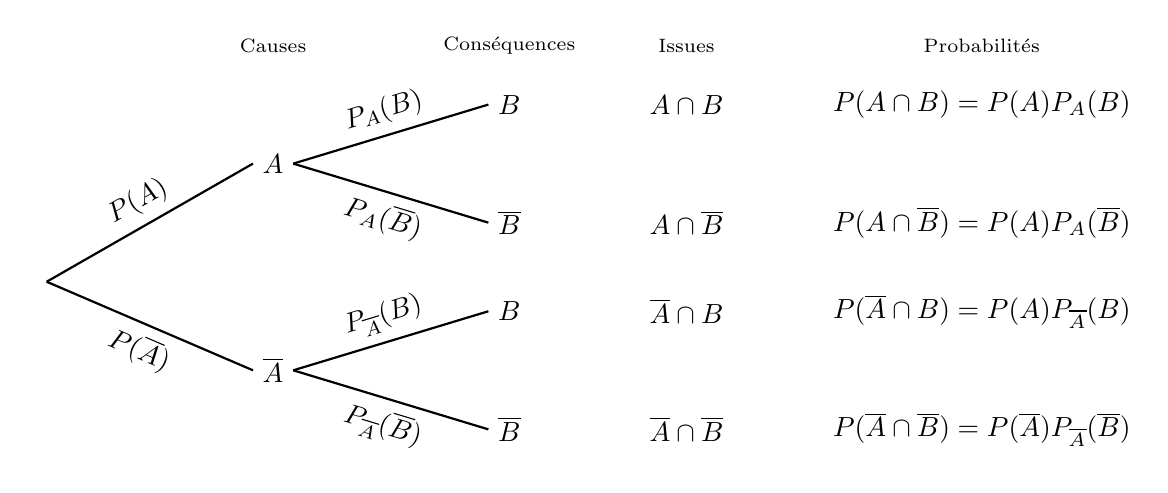
\begin{tikzpicture}[xscale=1,yscale=1]
		% Styles (MODIFIABLES)
		\tikzstyle{fleche}=[-,>=latex,thick]
		\tikzstyle{noeud}=[rounded corners=5pt]
		\tikzstyle{feuille}=[]
		\tikzstyle{commentaire}=[black]
		% Dimensions (MODIFIABLES)
		\def\DistanceInterNiveaux{3}
		\def\DistanceInterFeuilles{1.5}
		% Dimensions calculées (NON MODIFIABLES)
		\def\NiveauA{(0)*\DistanceInterNiveaux}
		\def\NiveauB{(1.0)*\DistanceInterNiveaux}
		\def\NiveauC{(2.0)*\DistanceInterNiveaux}
		\def\NiveauD{(2.750)*\DistanceInterNiveaux}
		\def\NiveauE{(4.0)*\DistanceInterNiveaux}
		\def\InterFeuilles{(-1)*\DistanceInterFeuilles}
		% Noeuds (MODIFIABLES : Styles et Coefficients d'InterFeuilles)
		\node[commentaire] (epreuve1) at ({\NiveauB},{(0)*\InterFeuilles}) {\scriptsize Causes};
		\node[commentaire] (epreuve2) at ({\NiveauC},{(0)*\InterFeuilles}) {\scriptsize Conséquences}; 
		\node[commentaire] (issues) at ({\NiveauD},{(0)*\InterFeuilles}) {\scriptsize Issues};
		\node[commentaire] (probas) at ({\NiveauE},{(0)*\InterFeuilles}) {\scriptsize Probabilités};
		% 
		\node[noeud] (R) at ({\NiveauA},{(2.00)*\InterFeuilles}) {};
		\node[noeud] (Ra) at ({\NiveauB},{(1)*\InterFeuilles}) {$A$};
		\node[feuille] (Raa) at ({\NiveauC},{(0.5)*\InterFeuilles}) {$B$}; 
		\node[feuille] (Rab) at ({\NiveauC},{(1.5)*\InterFeuilles}) {$\overline{B}$}; 
		\node[noeud] (Rb) at ({\NiveauB},{(2.75)*\InterFeuilles}) {$\overline{A}$};
		\node[feuille] (Rba) at ({\NiveauC},{(2.25)*\InterFeuilles}) {$B$}; 
		\node[feuille] (Rbb) at ({\NiveauC},{(3.25)*\InterFeuilles}) {$\overline{B}$}; 
		%
		\node[commentaire] (I1) at ({\NiveauD},{(0.5)*\InterFeuilles}) {$A\cap B$}; 
		\node[commentaire] (I2) at ({\NiveauD},{(1.5)*\InterFeuilles}) {$A\cap \overline{B}$}; 
		\node[commentaire] (I3) at ({\NiveauD},{(2.25)*\InterFeuilles}) {$\overline{A}\cap B$}; 
		\node[commentaire] (I4) at ({\NiveauD},{(3.25)*\InterFeuilles}) {$\overline{A}\cap \overline{B}$};
		%
		\node[commentaire] (P1) at ({\NiveauE},{(0.5)*\InterFeuilles}) {$P(A\cap B)=P(A)P_A(B)$}; 
		\node[commentaire] (P2) at ({\NiveauE},{(1.5)*\InterFeuilles}){$P(A\cap \overline{B})=P(A)P_A(\overline{B})$}; 
		%	\draw (P2.east) node[anchor=west, commentaire] {Faux négatif};
		\node[commentaire] (P3) at ({\NiveauE},{(2.25)*\InterFeuilles}){$P(\overline{A}\cap B)=P(A)P_{\overline{A}}(B)$}; 
		%	\draw (P3.east) node[anchor=west, commentaire] {Faux positif};
		\node[commentaire] (P4) at ({\NiveauE},{(3.25)*\InterFeuilles}) {$P(\overline{A}\cap \overline{B})=P(\overline{A})P_{\overline{A}}(\overline{B})$}; 
		%	\draw[ ultra thick] ({\NiveauE-1},{(3.55)*\InterFeuilles}) -- ({\NiveauE+1},{(3.55)*\InterFeuilles}) ;
		%	\node[commentaire] (P5) at ({\NiveauE},{(3.75)*\InterFeuilles})  {\textbf{Total}$=\ldots $}; 
		% Arcs (MODIFIABLES : Styles)
		\draw[fleche] (R.east)--(Ra.west) node[midway, above,sloped]{$P(A)$};
		\draw[fleche] (Ra.east)--(Raa.west) node[midway, above,sloped]{$P_A(B)$};
		\draw[fleche] (Ra.east)--(Rab.west) node[midway, below,sloped]{$P_A(\overline{B})$};
		\draw[fleche] (R.east)--(Rb.west) node[midway, below,sloped]{$P(\overline{A})$};
		\draw[fleche] (Rb.east)--(Rba.west) node[midway, above,sloped]{$P_{\overline{A}}(B)$};
		\draw[fleche] (Rb.east)--(Rbb.west) node[midway, below,sloped]{$P_{\overline{A}}(\overline{B})$};
	\end{tikzpicture}
	\caption{Un arbre de probabilité pour modéliser une situation mélant 2 événements $A$ et $B$.}
\end{figure*}
\begin{proposition}[Formule des probabilités totales (cas simple)] Pour calculer $P(B)$ dans le cas simple ci-dessus :
	\setlength{\abovedisplayskip}{3pt}
	\setlength{\belowdisplayskip}{3pt}
	\begin{align*}
		P(B)& = P(B\cap A) + P(B\cap \overline{A})\\
		& = P(A)P_A(B)  + P(\overline{A})P_{\overline{A}}(B)
	\end{align*} 
\end{proposition}
%  \begin{corollary}[Formule de Bayes] (Hors. Programme).\\
	%  	\setlength{\abovedisplayskip}{3pt}
	%  	\setlength{\belowdisplayskip}{3pt}
	%$$
	%  		P_B(A)  = \frac{P(A)P_A(B)}{ P(A)P_A(B)  + P(\overline{A})P_{\overline{A}}(B)}
	%$$
	%  	\end{corollary}

%----------------------------------------------------------------------------------------

\newpage 

 
\begin{definition}[partition de $\Omega$] 
	Les événements $A_1, A_2, ..., A_n$ pour $n \geqslant 1$ forment une partition de  $\Omega$  si   : 
	\begin{enumerate}[label=\textbullet, leftmargin=*]
		\item $A_1 \cup A_2 \cup ... \cup A_n = \Omega$;
		\item Les événements sont disjoints deux à deux : 
		\setlength{\abovedisplayskip}{3pt}
		\setlength{\belowdisplayskip}{3pt}
		$$ \text{pour tout $i,j \leqslant n$ avec $i\neq j$} \qquad A_i\cap A_j=\emptyset
		$$
	\end{enumerate}
\end{definition} 
\begin{proposition}[Probabilités totales] (forme générale) Pour la partition $(A_i)$ et un événement $E$ :
	\setlength{\abovedisplayskip}{3pt}
	\setlength{\belowdisplayskip}{3pt}
	$$
	P(E)=\sum_i P(A_i) P_{A_i}(E)
	$$
\end{proposition}

\begin{figure}[!h] 
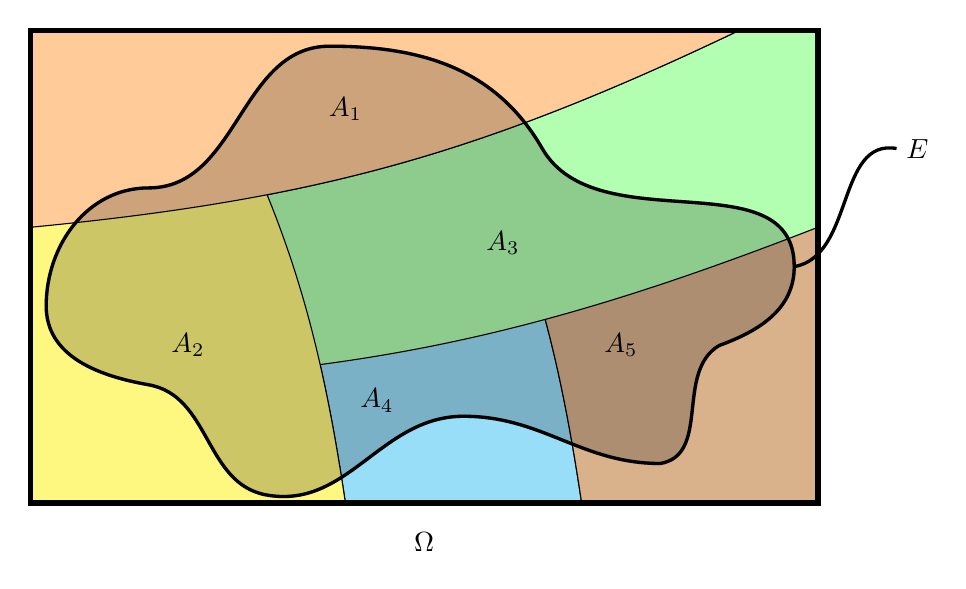
\begin{tikzpicture}
	\path
	coordinate (aux0) at (0,1.5)
	coordinate (aux1) at (0,3.5)
	coordinate (aux2) at (10,3.5)
	coordinate (aux3) at (9,6)
	coordinate (aux4) at (4,0)
	coordinate (aux5) at (7,0)
	coordinate (aux6) at (2,6)
	coordinate (aux7) at (5,6)
	coordinate (esp1) at (0.2,2.5)
	coordinate (esp2) at (1.5,1.5)
	coordinate (esp3) at (3,0.1)
	coordinate (esp4) at (5.5,1.1)
	coordinate (esp5) at (8,0.5)
	coordinate (esp6) at (8.75,2)
	coordinate (esp7) at (9.7,3)
	coordinate (esp8) at (6.5,4.5)
	coordinate (esp9) at (3.8,5.8)
	coordinate (esp10) at (1.5,4)
	;
%	\draw[line width=0.8pt]
%	(esp1) to[out=-90,in=170]
%	(esp2) to[out=-10,in=170]
%	(esp3) to[out=-10,in=180]
%	(esp4) to[out=0,in=180]
%	(esp5) to[out=10,in=-150]
%	(esp6) to[out=20,in=-90]
%	(esp7) to[out=90,in=-60]
%	(esp8) to[out=120,in=0]
%	(esp9) to[out=180,in=0]
%	(esp10) to[out=180,in=90]
%	cycle;     
%	\clip   
%	(esp1) to[out=-90,in=170]
%	(esp2) to[out=-10,in=170]
%	(esp3) to[out=-10,in=180]
%	(esp4) to[out=0,in=180]
%	(esp5) to[out=10,in=-150]
%	(esp6) to[out=20,in=-90]
%	(esp7) to[out=90,in=-60]
%	(esp8) to[out=120,in=0]
%	(esp9) to[out=180,in=0]
%	(esp10) to[out=180,in=90]
%	cycle;    
	\filldraw[fill=cyan!40]
	(aux4) to[bend right=10]
	(aux6) --
	(aux7) to[bend left=10]
	(aux5) -- cycle;
	\filldraw[fill=brown!60]
	(aux5) to[bend right=10]
	(aux7) --
	(10,6) --
	(10,0) -- cycle;
	\filldraw[fill=green!30]
	(aux0) -- 
	(aux1) to[bend right=10]
	(aux3) --
	(10,6) -- 
	(aux2) to[bend left=10] cycle;
	\filldraw[fill=yellow!50]
	(0,0) -- 
	(aux4) to[bend right=10]
	(aux6) --
	(0,6) -- 
	(0,0) -- cycle;
	\filldraw[fill=orange!40]
	(0,6) -- 
	(aux1) to[bend right=10]
	(aux3) --
	(0,6) -- cycle; 
\filldraw[line width=1.2pt, opacity=0.2]
	(esp1) to[out=-90,in=170]
	(esp2) to[out=-10,in=170]
	(esp3) to[out=-10,in=180]
	(esp4) to[out=0,in=180]
	(esp5) to[out=10,in=-150]
	(esp6) to[out=20,in=-90]
	(esp7) to[out=90,in=-60]
	(esp8) to[out=120,in=0]
	(esp9) to[out=180,in=0]
	(esp10) to[out=180,in=90]
	cycle; 
\draw[line width=1.2pt]
(esp1) to[out=-90,in=170]
(esp2) to[out=-10,in=170]
(esp3) to[out=-10,in=180]
(esp4) to[out=0,in=180]
(esp5) to[out=10,in=-150]
(esp6) to[out=20,in=-90]
(esp7) to[out=90,in=-60]
(esp8) to[out=120,in=0]
(esp9) to[out=180,in=0]
(esp10) to[out=180,in=90]
cycle; 
\draw[line width=2pt]
(10,0) --
(10,6) -- 
(0,6) -- 
(0,0) -- cycle; 
	\node at (4,5) {$A_1$};  
	\node at (2,2) {$A_2$};  
	\node at (6,3.3) {$A_3$};  
	\node at (4.4,1.3) {$A_4$};  
	\node at (7.5,2) {$A_5$};  
	\node at (5,-0.5) {$\Omega$};  
	\node[right] at (11,4.5) {$E$}; 
\draw[line width=1.2pt]
(esp7) to[out=10,in=170]  
(11,4.5) ;
\end{tikzpicture}
\parbox{1\linewidth}{
$P(E)=P(A_1)P_{A_1}(E)+P(A_2)P_{A_2}(E)+P(A_3)P_{A_3}(E)+\ldots$
}
\caption{Partition de l'univers $\Omega$ en 5 événements : $A_1\cup A_2\cup A_3\cup A_4\cup A_5=\Omega$}
\end{figure}


%----------------------------------------------------------------------------------------
%	EXERCICES
%----------------------------------------------------------------------------------------

\newpage 
\loadgeometry{widelayout}  
\pagestyle{scrheadings} % Print headers again  
\KOMAoptions{
	headwidth=textwithmarginpar,
	headsepline=true,
	headsepline= 0.5pt,
	footwidth=textwithmarginpar,
} 
\onehalfspacing
\subsection{Exercices : formule des probabilités composées et arbres de probabilités}


\begin{exercise}  Complétez\vspace{-.75em}
	\begin{spacing}{2}
		\begin{enumerate}[label=\arabic*), leftmargin=*]
			\item $B\subset A$, $P_B(A)=\frac{P(\ldots \cap \ldots)}{P(\ldots)}=\frac{P(\ldots)}{P(\ldots)}=\dotfill $
			\item  $P(A)=\numprint{0.22}$, $P(B)=\numprint{0.42}$ et $P(A\cap B)=\numprint{0.0836}$.\\
			$P_B(A)=\frac{P(\ldots\cap \ldots)}{P(\ldots)}=\dotfill $\\
			$P_B(A)=P(B)$, donc  l'événement \dotfill est indépendant de l'événement \dotfill
			\item $P(C)=\numprint{0.59}$, $P(D)=\numprint{0.25}$ et $P(C\cap D)=\numprint{0.1062}$.\\
			$P_C(D)=\frac{P(\ldots\cap \ldots)}{P(\ldots)}=\dotfill $\\
			$P_C(D)\ldots P(D)$, donc  l'événement \dotfill est défaborable à l'événement \dotfill
			\item $P(A)=\numprint{0.72}$, $P(B)=\numprint{0.3}$ et $P_B(A)=\numprint{0.75}$\\
			$P(A\cap B)=P(\ldots) P_{\ldots} (\ldots) =$\dotfill \\
			$P_A(B)=\frac{P(\ldots\cap \ldots)}{P(\ldots)}=\dotfill $
			\item $P(C)=\numprint{0.5}$, $P(D)=\numprint{0.12}$ et $P_C(D)=\numprint{0.09}$\\
			$P(C\cap D)=P(\ldots) P_{\ldots} (\ldots) =$\dotfill \\
			$P_D(C)=\frac{P(\ldots\cap \ldots)}{P(\ldots)}=\dotfill $
			\item $P_A(\ldots)+P_A(\ldots)= 1$
		\end{enumerate}
	\end{spacing}\vspace{-0.75em}
\end{exercise}  
\begin{exercise}[Entrainement formules]
	Dans chacun des cas suivants, calculer les probabilités demandées.
	\begin{enumerate}[label=\arabic*),leftmargin=*]
		\item 	$P(A)=\numprint{0.75}$, $P(B)=\numprint{0.54}$ et $P(A\cap B)=\numprint{0.405}$. Calculer $P_A(B)$.
		\item $P(A)=\numprint{0.77}$, $P(B)=\numprint{0.19}$ et $P_A(B)=\numprint{0.13}$. Calculer $P_B(A)$. %0.53
		\item $P(A)=\numprint{0.35}$ et $P_A(B)=\numprint{0.42}$ et $P_{\overline{A}}(\overline{B})=\numprint{0.82}$. Calculer $P(A\cap B)$  et $P_A(\overline{B})$. 
		\item $P(A)=\numprint{0.4}$, $P(B)=\numprint{0.17}$ et $P_B(A)=\numprint{0.24}$. Calculer $P_A(B)$. %0.1
		\item $P(A\cap B)=\numprint{0.18}$ et $P_A(B)=\numprint{0.6}$. Calculer $P(A)$.
	\end{enumerate}
\end{exercise}
\begin{exercise} $P(L)=\numprint{0.17}$, $P(B)=\numprint{0.12}$ et $P(L\cap M)=\numprint{0.0204}$. Montrer que $M$ est indépendant de $L$. 
\end{exercise}
\begin{exercise} $P(X)=\numprint{0.3}$, $P(Y)=\numprint{0.42}$ et $P(X\cup Y)=\numprint{0.594}$. Montrer que $Y$ est indépendant de $X$. 
\end{exercise} 
\begin{exercise} Une batterie de missiles a une probabilité de $\numprint{0.75}$ d'atteindre une cible. La batterie a une probabilité de $\numprint{0.65}$ d'atteindre deux cibles successives. Quelle est la probabilité d'atteindre la deuxième cible sachant que la première cible est atteinte ?
\end{exercise}
\begin{exercise} Quark a $80\%$ de chance de réussir son premier examen de Maths, et $45\%$ de chance de réussir les deux premiers examens de maths. Quelle est la probabilité de réussir le second examen sachant qu'il a réussi le premier examen ? 
\end{exercise}
%----------------------------------------------------------------------------------------

\newpage 
\begin{example}[interpéter et exploiter un arbre de probabilité] Soit un univers $\Omega$ et un loi de probabilité $P$, et les événements $A$ et $B$ modélisé par l'arbre ci-dessous : \\
	%\begin{figure*}[!h] 
	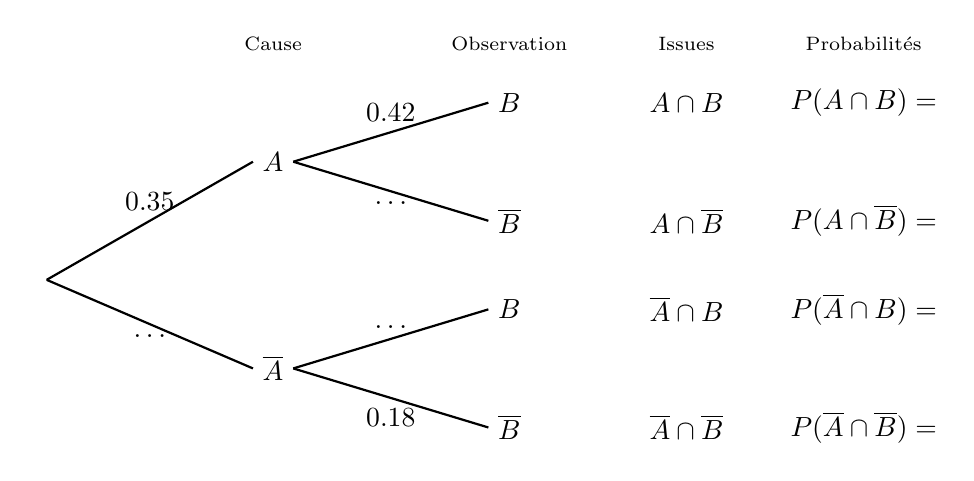
\begin{tikzpicture}[xscale=1,yscale=1]
		% Styles (MODIFIABLES)
		\tikzstyle{fleche}=[-,>=latex,thick]
		\tikzstyle{noeud}=[rounded corners=5pt]
		\tikzstyle{feuille}=[]
		\tikzstyle{commentaire}=[black]
		% Dimensions (MODIFIABLES)
		\def\DistanceInterNiveaux{3}
		\def\DistanceInterFeuilles{1.5}
		% Dimensions calculées (NON MODIFIABLES)
		\def\NiveauA{(0)*\DistanceInterNiveaux}
		\def\NiveauB{(1.0)*\DistanceInterNiveaux}
		\def\NiveauC{(2.0)*\DistanceInterNiveaux}
		\def\NiveauD{(2.750)*\DistanceInterNiveaux}
		\def\NiveauE{(3.5)*\DistanceInterNiveaux}
		\def\InterFeuilles{(-1)*\DistanceInterFeuilles}
		% Noeuds (MODIFIABLES : Styles et Coefficients d'InterFeuilles)
		\node[commentaire] (epreuve1) at ({\NiveauB},{(0)*\InterFeuilles}) {\scriptsize Cause};
		\node[commentaire] (epreuve2) at ({\NiveauC},{(0)*\InterFeuilles}) {\scriptsize Observation}; 
		\node[commentaire] (issues) at ({\NiveauD},{(0)*\InterFeuilles}) {\scriptsize Issues};
		\node[commentaire] (probas) at ({\NiveauE},{(0)*\InterFeuilles}) {\scriptsize Probabilités};
		% 
		\node[noeud] (R) at ({\NiveauA},{(2.00)*\InterFeuilles}) {};
		\node[noeud] (Ra) at ({\NiveauB},{(1)*\InterFeuilles}) {$A$};
		\node[feuille] (Raa) at ({\NiveauC},{(0.5)*\InterFeuilles}) {$B$}; 
		\node[feuille] (Rab) at ({\NiveauC},{(1.5)*\InterFeuilles}) {$\overline{B}$}; 
		\node[noeud] (Rb) at ({\NiveauB},{(2.75)*\InterFeuilles}) {$\overline{A}$};
		\node[feuille] (Rba) at ({\NiveauC},{(2.25)*\InterFeuilles}) {$B$}; 
		\node[feuille] (Rbb) at ({\NiveauC},{(3.25)*\InterFeuilles}) {$\overline{B}$}; 
		%
		\node[commentaire] (I1) at ({\NiveauD},{(0.5)*\InterFeuilles}) {$A\cap B$}; 
		\node[commentaire] (I2) at ({\NiveauD},{(1.5)*\InterFeuilles}) {$A\cap \overline{B}$}; 
		\node[commentaire] (I3) at ({\NiveauD},{(2.25)*\InterFeuilles}) {$\overline{A}\cap B$}; 
		\node[commentaire] (I4) at ({\NiveauD},{(3.25)*\InterFeuilles}) {$\overline{A}\cap \overline{B}$};
		%
		\node[commentaire] (P1) at ({\NiveauE},{(0.5)*\InterFeuilles}) {$P(A\cap B)= $}; 
		\node[commentaire] (P2) at ({\NiveauE},{(1.5)*\InterFeuilles}){$P(A\cap \overline{B})= $}; 
		%	\draw (P2.east) node[anchor=west, commentaire] {Faux négatif};
		\node[commentaire] (P3) at ({\NiveauE},{(2.25)*\InterFeuilles}){$P(\overline{A}\cap B)= $}; 
		%	\draw (P3.east) node[anchor=west, commentaire] {Faux positif};
		\node[commentaire] (P4) at ({\NiveauE},{(3.25)*\InterFeuilles}) {$P(\overline{A}\cap \overline{B})=$}; 
		%		\draw[ ultra thick] ({\NiveauE-1},{(3.55)*\InterFeuilles}) -- ({\NiveauE+1},{(3.55)*\InterFeuilles}) ;
		%		\node[commentaire] (P5) at ({\NiveauE},{(3.75)*\InterFeuilles})  {\textbf{Total}$=\ldots $}; 
		
		% Arcs (MODIFIABLES : Styles)
		\draw[fleche] (R.east)--(Ra.west) node[midway, above]{$0.35$};
		\draw[fleche] (Ra.east)--(Raa.west) node[midway, above]{$0.42$};
		\draw[fleche] (Ra.east)--(Rab.west) node[midway, below]{$\ldots$};
		\draw[fleche] (R.east)--(Rb.west) node[midway, below]{$\ldots$};
		\draw[fleche] (Rb.east)--(Rba.west) node[midway, above]{$\ldots$};
		\draw[fleche] (Rb.east)--(Rbb.west) node[midway, below]{$0.18$};
	\end{tikzpicture} 
	%\hspace{6cm} 
	%\end{figure*}
	\begin{enumerate}[label={\arabic*)},leftmargin=*]
		\item \textbf{Interpétation des données :} $P(\ldots)= 0.35$ ; $P_{\ldots}(\ldots)=0.42$ et $P_{\ldots}(\ldots)=0.18$.
		\item \textbf{Compléter l'arbre de probablité} :\\
		\noindent
		\parbox{0.33\linewidth}{
			$\begin{WithArrows}
				P(\overline{A})& = 1- P(\ldots )\rule{0pt}{1.6em} \\
				& =\rule{0pt}{1.6em} \\
				& =	\rule{0pt}{1.6em}
			\end{WithArrows}$\hfill 
		}\hfill 
		\parbox{0.33\linewidth}{
			$\begin{WithArrows}
				P_A(\overline{B})& = 1- P_{\ldots}(\ldots )\rule{0pt}{1.6em} \\
				& =\rule{0pt}{1.6em} \\
				& =	\rule{0pt}{1.6em}
			\end{WithArrows}$\hfill
		}\hfill 
		\parbox{0.33\linewidth}{
			$\begin{WithArrows}
				P_{\overline{A}}(\overline{B})& = 1- P_{\ldots}(\ldots ) \rule{0pt}{1.6em}\\
				& = \rule{0pt}{1.6em}\\
				& =	\rule{0pt}{1.6em}
			\end{WithArrows}$\hfill
		}  
		\item \textbf{Calculer les probablités des issues} à l'aide de la formule des probabilités composés \\
		\noindent
		\parbox{0.48\linewidth}{
			$\begin{WithArrows}
				P(A\cap B)& =P(\ldots)P_{\ldots}(\ldots) =\rule{0pt}{1.6em}  \\
				& =  \rule{0pt}{1.6em}
			\end{WithArrows}$\hfill 
		}\hfill 
		\parbox{0.48\linewidth}{
			$\begin{WithArrows}
				P(A\cap\overline{B})& =P(\ldots)P_{\ldots}(\ldots)= \rule{0pt}{1.6em}\\
				& =  \rule{0pt}{1.6em}
			\end{WithArrows}$\hfill
		}\\ 
		\parbox{0.48\linewidth}{
			$\begin{WithArrows}
				P(\overline{A}\cap B)& =  \rule{0pt}{1.6em} \\
				& =  \rule{0pt}{1.6em}
			\end{WithArrows}$\hfill
		} \hfill 
		\parbox{0.48\linewidth}{
			$\begin{WithArrows}
				P(\overline{A}\cap\overline{B})& =P(\ldots)P_{\ldots}(\ldots)= \rule{0pt}{1.6em}\\
				& =  \rule{0pt}{1.6em}
			\end{WithArrows}$\hfill
		} 
		\item \textbf{Calculer les probablités totales :} arrondir à $10^{-2}$\\
		\parbox{0.58\linewidth}{
			$\begin{WithArrows}
				P(B)& =P(\ldots\cap \ldots ) + P(\ldots\cap \ldots)= \rule{0pt}{1.6em}\\
				& =  \rule{0pt}{1.6em}
			\end{WithArrows}$ 
		}  
		\parbox{0.38\linewidth}{
			$\begin{WithArrows}
				P(\overline{B})& = \rule{0pt}{1.6em} \\
				& =  \rule{0pt}{1.6em}
			\end{WithArrows}$ 
		} 	
		\item \textbf{Inverser l'arbre :} calculer la probabilité sachant l'observation, de la cause\\
		\parbox{0.48\linewidth}{
			$\begin{WithArrows}
				P_B(A)& =  \rule{0pt}{1.6em}\\
				& =  \rule{0pt}{1.6em}
			\end{WithArrows}$ 
		} 	  
		\parbox{0.48\linewidth}{
			$\begin{WithArrows}
				P_{\overline{B}}(\overline{A})& = \rule{0pt}{1.6em}\\
				& =  \rule{0pt}{1.6em}
			\end{WithArrows}$ 
		} \\
		\item  \textbf{Représenter l'arbre inverse}  \\
		\parbox{0.38\linewidth}{
			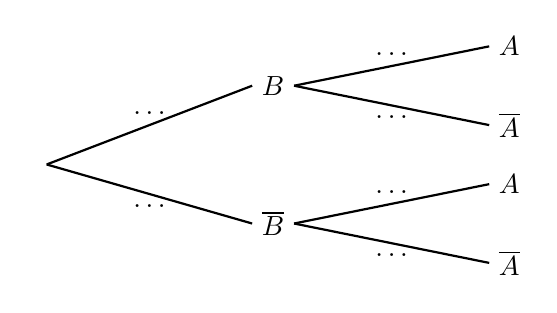
\begin{tikzpicture}[xscale=1,yscale=1]
				% Styles (MODIFIABLES)
				\tikzstyle{fleche}=[-,>=latex,thick]
				\tikzstyle{noeud}=[rounded corners=5pt]
				\tikzstyle{feuille}=[]
				\tikzstyle{commentaire}=[black]
				% Dimensions (MODIFIABLES)
				\def\DistanceInterNiveaux{3}
				\def\DistanceInterFeuilles{1.0}
				% Dimensions calculées (NON MODIFIABLES)
				\def\NiveauA{(0)*\DistanceInterNiveaux}
				\def\NiveauB{(1.0)*\DistanceInterNiveaux}
				\def\NiveauC{(2.0)*\DistanceInterNiveaux}
				\def\NiveauD{(2.750)*\DistanceInterNiveaux}
				\def\NiveauE{(3.5)*\DistanceInterNiveaux}
				\def\InterFeuilles{(-1)*\DistanceInterFeuilles}
				% Noeuds (MODIFIABLES : Styles et Coefficients d'InterFeuilles)
				%	\node[commentaire] (epreuve1) at ({\NiveauB},{(0)*\InterFeuilles}) {\scriptsize Observation};
				%	\node[commentaire] (epreuve2) at ({\NiveauC},{(0)*\InterFeuilles}) {\scriptsize Cause}; 
				%	\node[commentaire] (issues) at ({\NiveauD},{(0)*\InterFeuilles}) {\scriptsize Issues};
				%	\node[commentaire] (probas) at ({\NiveauE},{(0)*\InterFeuilles}) {\scriptsize Probabilités};
				% 
				\node[noeud] (R) at ({\NiveauA},{(2.00)*\InterFeuilles}) {};
				\node[noeud] (Ra) at ({\NiveauB},{(1)*\InterFeuilles}) {$B$};
				\node[feuille] (Raa) at ({\NiveauC},{(0.5)*\InterFeuilles}) {$A$}; 
				\node[feuille] (Rab) at ({\NiveauC},{(1.5)*\InterFeuilles}) {$\overline{A}$}; 
				\node[noeud] (Rb) at ({\NiveauB},{(2.75)*\InterFeuilles}) {$\overline{B}$};
				\node[feuille] (Rba) at ({\NiveauC},{(2.25)*\InterFeuilles}) {$A$}; 
				\node[feuille] (Rbb) at ({\NiveauC},{(3.25)*\InterFeuilles}) {$\overline{A}$}; 
				%
				%	\node[commentaire] (I1) at ({\NiveauD},{(0.5)*\InterFeuilles}) {$A\cap B$}; 
				%	\node[commentaire] (I2) at ({\NiveauD},{(1.5)*\InterFeuilles}) {$A\cap \overline{B}$}; 
				%	\node[commentaire] (I3) at ({\NiveauD},{(2.25)*\InterFeuilles}) {$\overline{A}\cap B$}; 
				%	\node[commentaire] (I4) at ({\NiveauD},{(3.25)*\InterFeuilles}) {$\overline{A}\cap \overline{B}$};
				%	%
				%	\node[commentaire] (P1) at ({\NiveauE},{(0.5)*\InterFeuilles}) {$P(A\cap B)= $}; 
				%	\node[commentaire] (P2) at ({\NiveauE},{(1.5)*\InterFeuilles}){$P(A\cap \overline{B})= $}; 
				%	%	\draw (P2.east) node[anchor=west, commentaire] {Faux négatif};
				%	\node[commentaire] (P3) at ({\NiveauE},{(2.25)*\InterFeuilles}){$P(\overline{A}\cap B)= $}; 
				%	%	\draw (P3.east) node[anchor=west, commentaire] {Faux positif};
				%	\node[commentaire] (P4) at ({\NiveauE},{(3.25)*\InterFeuilles}) {$P(\overline{A}\cap \overline{B})=$}; 
				%	%		\draw[ ultra thick] ({\NiveauE-1},{(3.55)*\InterFeuilles}) -- ({\NiveauE+1},{(3.55)*\InterFeuilles}) ;
				%	%		\node[commentaire] (P5) at ({\NiveauE},{(3.75)*\InterFeuilles})  {\textbf{Total}$=\ldots $}; 
				%	
				% Arcs (MODIFIABLES : Styles)
				\draw[fleche] (R.east)--(Ra.west) node[midway, above]{$\ldots$};
				\draw[fleche] (Ra.east)--(Raa.west) node[midway, above]{$\ldots$};
				\draw[fleche] (Ra.east)--(Rab.west) node[midway, below]{$\ldots$};
				\draw[fleche] (R.east)--(Rb.west) node[midway, below]{$\ldots$};
				\draw[fleche] (Rb.east)--(Rba.west) node[midway, above]{$\ldots$};
				\draw[fleche] (Rb.east)--(Rbb.west) node[midway, below]{$\ldots$};
			\end{tikzpicture} 
		}
		\hfill 
		\parbox{0.60\linewidth}{
			\begin{eBox} 
				\noindent\footnotesize 
				\faHeart 	Les chemins correspondent à des événements incompatibles. \\ 
				\textbullet  	La probabilité d'un événement auquel conduit un chemin est égale
				au produit des probabilités rencontrées le long de ce chemin. \\
				\textbullet	La somme des probabilités des branches issues d'un même noeud vaut 1.
			\end{eBox} 
		}
	\end{enumerate} 
\end{example}

%----------------------------------------------------------------------------------------

\newpage  
\begin{exercise}[] $0.1\%$ de la population est atteinte du cancer des poumons ($C$). $90\%$ des personnes atteintes de cancer sont des fumeurs ($F$). $21\%$ de ceux qui n'ont pas de cancer sont des fumeurs.  
	\begin{enumerate}[label={\arabic*)},leftmargin=*]
		\item Identifier les probabilités données dans l'énoncé et ajouter les dans l'arbre de probabilité \\
		\rule{0pt}{1.8em}$P(\ldots)=$ \hfill $P_{\ldots}(\ldots)=$\hfill $P_{\ldots}(\ldots)=$\hfill \null \medskip\\
		\parbox{0.5\linewidth}{
			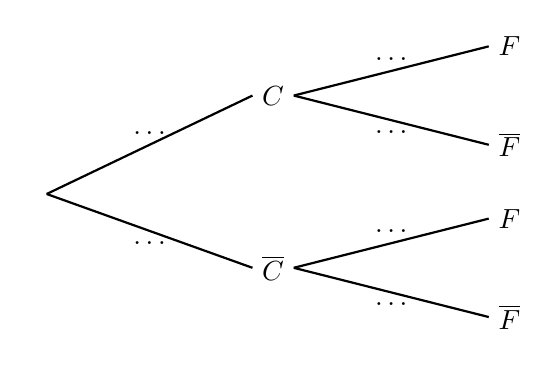
\begin{tikzpicture}[xscale=1,yscale=1]
				% Styles (MODIFIABLES)
				\tikzstyle{fleche}=[-,>=latex,thick]
				\tikzstyle{noeud}=[rounded corners=5pt]
				\tikzstyle{feuille}=[]
				\tikzstyle{commentaire}=[black]
				% Dimensions (MODIFIABLES)
				\def\DistanceInterNiveaux{3}
				\def\DistanceInterFeuilles{1.25}
				% Dimensions calculées (NON MODIFIABLES)
				\def\NiveauA{(0)*\DistanceInterNiveaux}
				\def\NiveauB{(1.0)*\DistanceInterNiveaux}
				\def\NiveauC{(2.0)*\DistanceInterNiveaux}
				\def\NiveauD{(2.750)*\DistanceInterNiveaux}
				\def\NiveauE{(3.5)*\DistanceInterNiveaux}
				\def\InterFeuilles{(-1)*\DistanceInterFeuilles}
				% Noeuds (MODIFIABLES : Styles et Coefficients d'InterFeuilles)
				%	\node[commentaire] (epreuve1) at ({\NiveauB},{(0)*\InterFeuilles}) {\scriptsize Observation};
				%	\node[commentaire] (epreuve2) at ({\NiveauC},{(0)*\InterFeuilles}) {\scriptsize Cause}; 
				%	\node[commentaire] (issues) at ({\NiveauD},{(0)*\InterFeuilles}) {\scriptsize Issues};
				%	\node[commentaire] (probas) at ({\NiveauE},{(0)*\InterFeuilles}) {\scriptsize Probabilités};
				% 
				\node[noeud] (R) at ({\NiveauA},{(2.00)*\InterFeuilles}) {};
				\node[noeud] (Ra) at ({\NiveauB},{(1)*\InterFeuilles}) {$C$};
				\node[feuille] (Raa) at ({\NiveauC},{(0.5)*\InterFeuilles}) {$F$}; 
				\node[feuille] (Rab) at ({\NiveauC},{(1.5)*\InterFeuilles}) {$\overline{F}$}; 
				\node[noeud] (Rb) at ({\NiveauB},{(2.75)*\InterFeuilles}) {$\overline{C}$};
				\node[feuille] (Rba) at ({\NiveauC},{(2.25)*\InterFeuilles}) {$F$}; 
				\node[feuille] (Rbb) at ({\NiveauC},{(3.25)*\InterFeuilles}) {$\overline{F}$}; 
				%
				%	\node[commentaire] (I1) at ({\NiveauD},{(0.5)*\InterFeuilles}) {$A\cap B$}; 
				%	\node[commentaire] (I2) at ({\NiveauD},{(1.5)*\InterFeuilles}) {$A\cap \overline{B}$}; 
				%	\node[commentaire] (I3) at ({\NiveauD},{(2.25)*\InterFeuilles}) {$\overline{A}\cap B$}; 
				%	\node[commentaire] (I4) at ({\NiveauD},{(3.25)*\InterFeuilles}) {$\overline{A}\cap \overline{B}$};
				%	%
				%	\node[commentaire] (P1) at ({\NiveauE},{(0.5)*\InterFeuilles}) {$P(A\cap B)= $}; 
				%	\node[commentaire] (P2) at ({\NiveauE},{(1.5)*\InterFeuilles}){$P(A\cap \overline{B})= $}; 
				%	%	\draw (P2.east) node[anchor=west, commentaire] {Faux négatif};
				%	\node[commentaire] (P3) at ({\NiveauE},{(2.25)*\InterFeuilles}){$P(\overline{A}\cap B)= $}; 
				%	%	\draw (P3.east) node[anchor=west, commentaire] {Faux positif};
				%	\node[commentaire] (P4) at ({\NiveauE},{(3.25)*\InterFeuilles}) {$P(\overline{A}\cap \overline{B})=$}; 
				%	%		\draw[ ultra thick] ({\NiveauE-1},{(3.55)*\InterFeuilles}) -- ({\NiveauE+1},{(3.55)*\InterFeuilles}) ;
				%	%		\node[commentaire] (P5) at ({\NiveauE},{(3.75)*\InterFeuilles})  {\textbf{Total}$=\ldots $}; 
				%	
				% Arcs (MODIFIABLES : Styles)
				\draw[fleche] (R.east)--(Ra.west) node[midway, above]{$\ldots$};
				\draw[fleche] (Ra.east)--(Raa.west) node[midway, above]{$\ldots$};
				\draw[fleche] (Ra.east)--(Rab.west) node[midway, below]{$\ldots$};
				\draw[fleche] (R.east)--(Rb.west) node[midway, below]{$\ldots$};
				\draw[fleche] (Rb.east)--(Rba.west) node[midway, above]{$\ldots$};
				\draw[fleche] (Rb.east)--(Rbb.west) node[midway, below]{$\ldots$};
			\end{tikzpicture} 
		}
		\hfill  
		\item Complétez l'arbre de probabilité en justifiant vos calculs :\\
		\noindent
		\parbox{0.33\linewidth}{
			$\begin{WithArrows}
				P(\ldots )& = 1- P(\ldots )\rule{0pt}{1.6em} \\
				& =\rule{0pt}{1.6em} \\
				& =	\rule{0pt}{1.6em}
			\end{WithArrows}$\hfill 
		}\hfill 
		\parbox{0.33\linewidth}{
			$\begin{WithArrows}
				P_{\ldots}(\ldots)& = 1- P_{\ldots}(\ldots )\rule{0pt}{1.6em} \\
				& =\rule{0pt}{1.6em} \\
				& =	\rule{0pt}{1.6em}
			\end{WithArrows}$\hfill
		}\hfill 
		\parbox{0.33\linewidth}{
			$\begin{WithArrows}
				P_{\ldots}(\ldots)& = 1- P_{\ldots}(\ldots ) \rule{0pt}{1.6em}\\
				& = \rule{0pt}{1.6em}\\
				& =	\rule{0pt}{1.6em}
			\end{WithArrows}$\hfill
		}  
		\item Calculer les probabilités des événements :\\
		$\begin{WithArrows}
			P(C \cap F) 	& = \rule{0pt}{1.8em}\\
			P(C\cap \overline{F}) 	& = \rule{0pt}{1.8em}\\
			P(\overline{C}\cap F) 	& = \rule{0pt}{1.8em}\\
			P(\overline{C}\cap \overline{F}) 	& = \rule{0pt}{1.8em}\\
			&
		\end{WithArrows}$ 
		\item Calculer la probabilité d'être un fumeur.\\
		$\begin{WithArrows}
			P(F) 	&= P(\ldots \cap \ldots) + P(\ldots\cap \ldots ) =  \rule{0pt}{1.6em} \\
			&
		\end{WithArrows}$ 		
		\item Calculer la probabilité d'avoir le cancer sachant qu'on est un fumeur.\\
		$\begin{WithArrows}
			P_{\ldots}(\ldots) 	&=   \rule{0pt}{1.6em} \\
			&
		\end{WithArrows}$ 
		\item Calculer la probabilité d'avoir le cancer sachant qu'on n'est pas un fumeur.\\
		$\begin{WithArrows}
			P_{\ldots}(\ldots) 	&=   \rule{0pt}{1.6em} \\
			&
		\end{WithArrows}$ 
		\item Par combien est multiplié le risque de développer un cancer des poumons si on est un fumeur ?
	\end{enumerate}
\end{exercise} 
%----------------------------------------------------------------------------------------

\newpage 

\begin{exercise}  
	Une urne opaque contient des boules rouges et des boules vertes indiscernables au toucher. 	On tire au hasard une boule de l'urne, on note sa couleur sans la remettre. On tire de nouveau une boule de l'urne et on note sa couleur. \\
	Soit les événement $R_1$   \og la boule tirée au premier est rouge\fg  et $R_2$   \og la boule tirée au second tour est rouge\fg. On modélise l'expérience aléatoire par l'arbre de probabilité incomplet ci-dessous.  \\
	\parbox{0.38\linewidth}{
		\begin{tikzpicture}[xscale=1,yscale=1]
			% Styles (MODIFIABLES)
			\tikzstyle{fleche}=[-,>=latex,thick]
			\tikzstyle{noeud}=[rounded corners=5pt]
			\tikzstyle{feuille}=[]
			\tikzstyle{commentaire}=[black]
			% Dimensions (MODIFIABLES)
			\def\DistanceInterNiveaux{3}
			\def\DistanceInterFeuilles{1.0}
			% Dimensions calculées (NON MODIFIABLES)
			\def\NiveauA{(0)*\DistanceInterNiveaux}
			\def\NiveauB{(1.0)*\DistanceInterNiveaux}
			\def\NiveauC{(2.0)*\DistanceInterNiveaux}
			\def\NiveauD{(2.750)*\DistanceInterNiveaux}
			\def\NiveauE{(3.5)*\DistanceInterNiveaux}
			\def\InterFeuilles{(-1)*\DistanceInterFeuilles}
			% Noeuds (MODIFIABLES : Styles et Coefficients d'InterFeuilles)
			%	\node[commentaire] (epreuve1) at ({\NiveauB},{(0)*\InterFeuilles}) {\scriptsize Observation};
			%	\node[commentaire] (epreuve2) at ({\NiveauC},{(0)*\InterFeuilles}) {\scriptsize Cause}; 
			%	\node[commentaire] (issues) at ({\NiveauD},{(0)*\InterFeuilles}) {\scriptsize Issues};
			%	\node[commentaire] (probas) at ({\NiveauE},{(0)*\InterFeuilles}) {\scriptsize Probabilités};
			% 
			\node[noeud] (R) at ({\NiveauA},{(2.00)*\InterFeuilles}) {};
			\node[noeud] (Ra) at ({\NiveauB},{(1)*\InterFeuilles}) {$R_1$};
			\node[feuille] (Raa) at ({\NiveauC},{(0.5)*\InterFeuilles}) {$R_2$}; 
			\node[feuille] (Rab) at ({\NiveauC},{(1.5)*\InterFeuilles}) {$\overline{R_2}$}; 
			\node[noeud] (Rb) at ({\NiveauB},{(2.75)*\InterFeuilles}) {$\overline{R_1}$};
			\node[feuille] (Rba) at ({\NiveauC},{(2.25)*\InterFeuilles}) {$R_2$}; 
			\node[feuille] (Rbb) at ({\NiveauC},{(3.25)*\InterFeuilles}) {$\overline{R_2}$}; 
			%
			%	\node[commentaire] (I1) at ({\NiveauD},{(0.5)*\InterFeuilles}) {$A\cap B$}; 
			%	\node[commentaire] (I2) at ({\NiveauD},{(1.5)*\InterFeuilles}) {$A\cap \overline{B}$}; 
			%	\node[commentaire] (I3) at ({\NiveauD},{(2.25)*\InterFeuilles}) {$\overline{A}\cap B$}; 
			%	\node[commentaire] (I4) at ({\NiveauD},{(3.25)*\InterFeuilles}) {$\overline{A}\cap \overline{B}$};
			%	%
			%	\node[commentaire] (P1) at ({\NiveauE},{(0.5)*\InterFeuilles}) {$P(A\cap B)= $}; 
			%	\node[commentaire] (P2) at ({\NiveauE},{(1.5)*\InterFeuilles}){$P(A\cap \overline{B})= $}; 
			%	%	\draw (P2.east) node[anchor=west, commentaire] {Faux négatif};
			%	\node[commentaire] (P3) at ({\NiveauE},{(2.25)*\InterFeuilles}){$P(\overline{A}\cap B)= $}; 
			%	%	\draw (P3.east) node[anchor=west, commentaire] {Faux positif};
			%	\node[commentaire] (P4) at ({\NiveauE},{(3.25)*\InterFeuilles}) {$P(\overline{A}\cap \overline{B})=$}; 
			%	%		\draw[ ultra thick] ({\NiveauE-1},{(3.55)*\InterFeuilles}) -- ({\NiveauE+1},{(3.55)*\InterFeuilles}) ;
			%	%		\node[commentaire] (P5) at ({\NiveauE},{(3.75)*\InterFeuilles})  {\textbf{Total}$=\ldots $}; 
			%	
			% Arcs (MODIFIABLES : Styles)
			\draw[fleche] (R.east)--(Ra.west) node[midway, above]{$\tfrac{2}{5}$};
			\draw[fleche] (Ra.east)--(Raa.west) node[midway, above]{$\tfrac{7}{19}$};
			\draw[fleche] (Ra.east)--(Rab.west) node[midway, below]{$\ldots$};
			\draw[fleche] (R.east)--(Rb.west) node[midway, below]{$\ldots$};
			\draw[fleche] (Rb.east)--(Rba.west) node[midway, above]{$\tfrac{8}{19}$};
			\draw[fleche] (Rb.east)--(Rbb.west) node[midway, below]{$\ldots$};
		\end{tikzpicture} 
	}
	\hfill 
	\parbox{0.6\linewidth}{
		
	}
	\begin{enumerate}[label={\arabic*)},leftmargin=*]
		\item Identifier les probabilités données dans l'arbre :\\
		\rule{0pt}{1.8em}$P(\ldots)=$ \hfill $P_{\ldots}(\ldots)=$\hfill $P_{\ldots}(\ldots)=$\hfill \null 
		\item Complétez l'arbre de probabilité en justifiant vos calculs :\\
		\noindent
		\parbox{0.33\linewidth}{
			$\begin{WithArrows}
				P(\ldots )& = 1- P(\ldots )\rule{0pt}{1.6em} \\
				& =\rule{0pt}{1.6em} \\
				& =	\rule{0pt}{1.6em}
			\end{WithArrows}$\hfill 
		}\hfill 
		\parbox{0.33\linewidth}{
			$\begin{WithArrows}
				P_{\ldots}(\overline{B})& = 1- P_{\ldots}(\ldots )\rule{0pt}{1.6em} \\
				& =\rule{0pt}{1.6em} \\
				& =	\rule{0pt}{1.6em}
			\end{WithArrows}$\hfill
		}\hfill 
		\parbox{0.33\linewidth}{
			$\begin{WithArrows}
				P_{\ldots}(\overline{B})& = 1- P_{\ldots}(\ldots ) \rule{0pt}{1.6em}\\
				& = \rule{0pt}{1.6em}\\
				& =	\rule{0pt}{1.6em}
			\end{WithArrows}$\hfill
		}  
		\item  Calculer la probabilité de tirer deux boules vertes. \\
		$\begin{WithArrows}
			P(\ldots\cap \ldots) 	& = \rule{0pt}{1.6em}\\
			&
		\end{WithArrows}$ 
		\item Calculer la probabilité que la boule tirée au second tour soit rouge.\\
		$\begin{WithArrows}
			P(\ldots ) &= P(\ldots \cap \ldots) + P(\ldots\cap \ldots ) =  \rule{0pt}{1.6em}\\
			& = \rule{0pt}{1.6em}\\
			&
		\end{WithArrows}$
		\item Calculer la probabilité de l'événement $A=$\og tirer deux boules de couleurs différentes\fg.\\
		$\begin{WithArrows}
			P(A) &= P(\ldots \cap \ldots) + P(\ldots\cap \ldots ) =  \rule{0pt}{1.6em}\\
			&   \rule{0pt}{1.6em} 
		\end{WithArrows}$  
	\end{enumerate}		 
\end{exercise}
\begin{exercise}	Une expérience aléatoire est modélisée par l'arbre ci-dessous. Calculer $P(B)$. \\
	\parbox{0.35\linewidth}{
		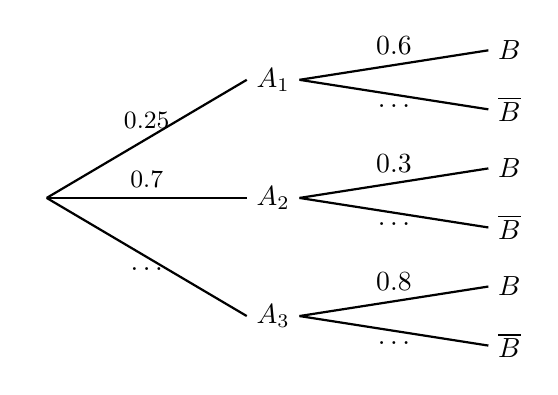
\begin{tikzpicture}[xscale=1,yscale=1]
			% Styles (MODIFIABLES)
			\tikzstyle{fleche}=[-,>=latex,thick]
			\tikzstyle{noeud}=[rounded corners=5pt]
			\tikzstyle{feuille}=[]
			\tikzstyle{commentaire}=[black]
			% Dimensions (MODIFIABLES)
			\def\DistanceInterNiveaux{3}
			\def\DistanceInterFeuilles{0.75}
			% Dimensions calculées (NON MODIFIABLES)
			\def\NiveauA{(0)*\DistanceInterNiveaux}
			\def\NiveauB{(1.0)*\DistanceInterNiveaux}
			\def\NiveauC{(2.0)*\DistanceInterNiveaux}
			\def\NiveauD{(2.750)*\DistanceInterNiveaux}
			\def\NiveauE{(3.5)*\DistanceInterNiveaux}
			\def\InterFeuilles{(-1)*\DistanceInterFeuilles}
			% Noeuds (MODIFIABLES : Styles et Coefficients d'InterFeuilles)
			%	\node[commentaire] (epreuve1) at ({\NiveauB},{(0)*\InterFeuilles}) {\scriptsize Observation};
			%	\node[commentaire] (epreuve2) at ({\NiveauC},{(0)*\InterFeuilles}) {\scriptsize Cause}; 
			%	\node[commentaire] (issues) at ({\NiveauD},{(0)*\InterFeuilles}) {\scriptsize Issues};
			%	\node[commentaire] (probas) at ({\NiveauE},{(0)*\InterFeuilles}) {\scriptsize Probabilités};
			% 
			\node[noeud] (R) at ({\NiveauA},{(3.5)*\InterFeuilles}) {};
			\node[noeud] (Ra) at ({\NiveauB},{(1.5)*\InterFeuilles}) {$A_1$};
			\node[feuille] (Raa) at ({\NiveauC},{(1)*\InterFeuilles}) {$B$}; 
			\node[feuille] (Rab) at ({\NiveauC},{(2)*\InterFeuilles}) {$\overline{B}$}; 
			\node[noeud] (Rb) at ({\NiveauB},{(3.5)*\InterFeuilles}) {${A_2}$};
			\node[feuille] (Rba) at ({\NiveauC},{(3)*\InterFeuilles}) {$B$}; 
			\node[feuille] (Rbb) at ({\NiveauC},{(4)*\InterFeuilles}) {$\overline{B}$}; 
			\node[noeud] (Rc) at ({\NiveauB},{(5.5)*\InterFeuilles}) {${A_3}$};
			\node[feuille] (Rca) at ({\NiveauC},{(5)*\InterFeuilles}) {$B$}; 
			\node[feuille] (Rcb) at ({\NiveauC},{(6)*\InterFeuilles}) {$\overline{B}$}; 
			%
			%	\node[commentaire] (I1) at ({\NiveauD},{(0.5)*\InterFeuilles}) {$A\cap B$}; 
			%	\node[commentaire] (I2) at ({\NiveauD},{(1.5)*\InterFeuilles}) {$A\cap \overline{B}$}; 
			%	\node[commentaire] (I3) at ({\NiveauD},{(2.25)*\InterFeuilles}) {$\overline{A}\cap B$}; 
			%	\node[commentaire] (I4) at ({\NiveauD},{(3.25)*\InterFeuilles}) {$\overline{A}\cap \overline{B}$};
			%	%
			%	\node[commentaire] (P1) at ({\NiveauE},{(0.5)*\InterFeuilles}) {$P(A\cap B)= $}; 
			%	\node[commentaire] (P2) at ({\NiveauE},{(1.5)*\InterFeuilles}){$P(A\cap \overline{B})= $}; 
			%	%	\draw (P2.east) node[anchor=west, commentaire] {Faux négatif};
			%	\node[commentaire] (P3) at ({\NiveauE},{(2.25)*\InterFeuilles}){$P(\overline{A}\cap B)= $}; 
			%	%	\draw (P3.east) node[anchor=west, commentaire] {Faux positif};
			%	\node[commentaire] (P4) at ({\NiveauE},{(3.25)*\InterFeuilles}) {$P(\overline{A}\cap \overline{B})=$}; 
			%	%		\draw[ ultra thick] ({\NiveauE-1},{(3.55)*\InterFeuilles}) -- ({\NiveauE+1},{(3.55)*\InterFeuilles}) ;
			%	%		\node[commentaire] (P5) at ({\NiveauE},{(3.75)*\InterFeuilles})  {\textbf{Total}$=\ldots $}; 
			%	
			% Arcs (MODIFIABLES : Styles)
			\draw[fleche] (R.east)--(Ra.west) node[midway, above]{\small$0.25$};
			\draw[fleche] (Ra.east)--(Raa.west) node[midway, above]{$0.6$};
			\draw[fleche] (Ra.east)--(Rab.west) node[midway, below]{$\ldots$};
			\draw[fleche] (R.east)--(Rb.west) node[midway, above]{\small$0.7$};
			\draw[fleche] (Rb.east)--(Rba.west) node[midway, above]{$0.3$};
			\draw[fleche] (Rb.east)--(Rbb.west) node[midway, below]{$\ldots$};
			\draw[fleche] (R.east)--(Rc.west) node[midway, below]{$\ldots$};
			\draw[fleche] (Rc.east)--(Rca.west) node[midway, above]{$0.8$};
			\draw[fleche] (Rc.east)--(Rcb.west) node[midway, below]{$\ldots$};
		\end{tikzpicture} 
	}
	\hfill 
	\parbox{0.63\linewidth}{
		$\begin{WithArrows}
			P(A_3)& = \rule{0pt}{1.6em}\\
			P(B)& = P(\ldots\cap \ldots)+P(\ldots\cap \ldots)+P(\ldots\cap \ldots) \rule{0pt}{1.6em}\\
			& =  P(\ldots) P_{\ldots}(  \ldots)+\rule{0pt}{1.6em} \\
			&=\rule{0pt}{1.6em} \\
			&=  
		\end{WithArrows}
		$
	} 
\end{exercise}
%----------------------------------------------------------------------------------------

\newpage 
\begin{exercise} 
	On dispose des informations suivantes sur une société :
	\begin{enumerate}[leftmargin=*, label=\textbullet]
		\item Elle comporte $40\%$ de cadres.
		\item  $20\%$ des cadres sont des femmes.
		\item Parmi les employés qui ne sont pas cadres, $60\%$ sont des femmes.
	\end{enumerate}  
	On prend au hasard la fiche d'un des employés et on considère les événements suivants :\\
	$C$: \og L'employé est un cadre \fg; \hspace*{5mm} $F$: \og L'employé est une femme\fg.
	\begin{enumerate}[leftmargin=*, label=\arabic*)]
		\item Traduire les données en termes de probabilités, en utilisant les événements $C$ et $F$.
		\item Représenter la situation par un arbre de probabilité.
		\item Calculer la probabilité pour qu'un employé interrogé soit une femme cadre.
	\end{enumerate}
\end{exercise}
\begin{exercise}[le taxi et le témoin] Un taxi est accusé de délit de fuite. Au tribunal le témoin confirme que le taxi était de couleur bleue. En ville, 85\% des taxis sont verts, et 15\% sont bleus. Le procureur teste la fiabilité du témoin dans des conditions de luminosité similaires à la nuit de l'incident. Il constate que le témoin identifie la bonne couleur dans 80\% des cas.\\
	On considère les événements suivants :\\
	$A$: \og le taxi est de couleur bleu\fg; \hspace*{5mm} $B$: \og le témoin affirme que la couleur du taxi est bleue\fg.
	\begin{enumerate}[leftmargin=*, label=\arabic*)]
		\item D'après l'énoncé, que vaut $P_A(B)$ ? $P_{\overline{A}}(B)$ ?
		\item Représenter la situation par un arbre de probabilité.
		\item Calculer la probabilité que le témoin affirme avoir vu un taxi bleu.
		\item Quelle est la probabilité que le taxi soit vert sachant que le témoin affirme il est bleu ?
	\end{enumerate}
\end{exercise}
\begin{exercise} 
	Un revendeur achète des pièces à trois fournisseurs $A$, $B$ et $C$. $60\%$ de son stock provient de $A$, $15\%$ de $B$ et le reste de $C$. $2\%$ des pièces venant de $A$ sont défectueuses, ainsi que $1\%$ de celles venant de $B$ et $0,5\%$ de celles qui viennent de $C$. \\
	\parbox{0.35\linewidth}{
		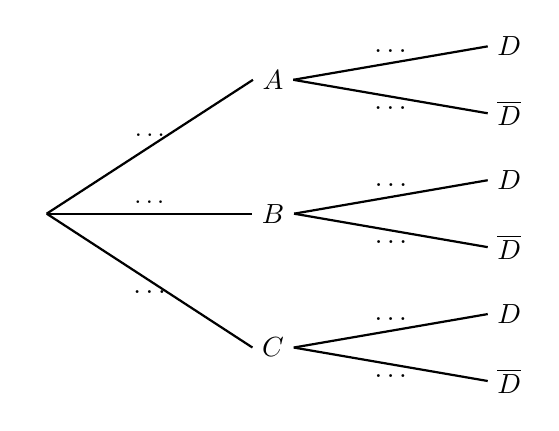
\begin{tikzpicture}[xscale=1,yscale=1]
			% Styles (MODIFIABLES)
			\tikzstyle{fleche}=[-,>=latex,thick]
			\tikzstyle{noeud}=[rounded corners=5pt]
			\tikzstyle{feuille}=[]
			\tikzstyle{commentaire}=[black]
			% Dimensions (MODIFIABLES)
			\def\DistanceInterNiveaux{3}
			\def\DistanceInterFeuilles{0.85}
			% Dimensions calculées (NON MODIFIABLES)
			\def\NiveauA{(0)*\DistanceInterNiveaux}
			\def\NiveauB{(1.0)*\DistanceInterNiveaux}
			\def\NiveauC{(2.0)*\DistanceInterNiveaux}
			\def\NiveauD{(2.750)*\DistanceInterNiveaux}
			\def\NiveauE{(3.5)*\DistanceInterNiveaux}
			\def\InterFeuilles{(-1)*\DistanceInterFeuilles}
			% Noeuds (MODIFIABLES : Styles et Coefficients d'InterFeuilles)
			%	\node[commentaire] (epreuve1) at ({\NiveauB},{(0)*\InterFeuilles}) {\scriptsize Observation};
			%	\node[commentaire] (epreuve2) at ({\NiveauC},{(0)*\InterFeuilles}) {\scriptsize Cause}; 
			%	\node[commentaire] (issues) at ({\NiveauD},{(0)*\InterFeuilles}) {\scriptsize Issues};
			%	\node[commentaire] (probas) at ({\NiveauE},{(0)*\InterFeuilles}) {\scriptsize Probabilités};
			% 
			\node[noeud] (R) at ({\NiveauA},{(3.5)*\InterFeuilles}) {};
			\node[noeud] (Ra) at ({\NiveauB},{(1.5)*\InterFeuilles}) {$A$};
			\node[feuille] (Raa) at ({\NiveauC},{(1)*\InterFeuilles}) {$D$}; 
			\node[feuille] (Rab) at ({\NiveauC},{(2)*\InterFeuilles}) {$\overline{D}$}; 
			\node[noeud] (Rb) at ({\NiveauB},{(3.5)*\InterFeuilles}) {${B}$};
			\node[feuille] (Rba) at ({\NiveauC},{(3)*\InterFeuilles}) {$D$}; 
			\node[feuille] (Rbb) at ({\NiveauC},{(4)*\InterFeuilles}) {$\overline{D}$}; 
			\node[noeud] (Rc) at ({\NiveauB},{(5.5)*\InterFeuilles}) {${C}$};
			\node[feuille] (Rca) at ({\NiveauC},{(5)*\InterFeuilles}) {$D$}; 
			\node[feuille] (Rcb) at ({\NiveauC},{(6)*\InterFeuilles}) {$\overline{D}$}; 
			%
			%	\node[commentaire] (I1) at ({\NiveauD},{(0.5)*\InterFeuilles}) {$A\cap B$}; 
			%	\node[commentaire] (I2) at ({\NiveauD},{(1.5)*\InterFeuilles}) {$A\cap \overline{B}$}; 
			%	\node[commentaire] (I3) at ({\NiveauD},{(2.25)*\InterFeuilles}) {$\overline{A}\cap B$}; 
			%	\node[commentaire] (I4) at ({\NiveauD},{(3.25)*\InterFeuilles}) {$\overline{A}\cap \overline{B}$};
			%	%
			%	\node[commentaire] (P1) at ({\NiveauE},{(0.5)*\InterFeuilles}) {$P(A\cap B)= $}; 
			%	\node[commentaire] (P2) at ({\NiveauE},{(1.5)*\InterFeuilles}){$P(A\cap \overline{B})= $}; 
			%	%	\draw (P2.east) node[anchor=west, commentaire] {Faux négatif};
			%	\node[commentaire] (P3) at ({\NiveauE},{(2.25)*\InterFeuilles}){$P(\overline{A}\cap B)= $}; 
			%	%	\draw (P3.east) node[anchor=west, commentaire] {Faux positif};
			%	\node[commentaire] (P4) at ({\NiveauE},{(3.25)*\InterFeuilles}) {$P(\overline{A}\cap \overline{B})=$}; 
			%	%		\draw[ ultra thick] ({\NiveauE-1},{(3.55)*\InterFeuilles}) -- ({\NiveauE+1},{(3.55)*\InterFeuilles}) ;
			%	%		\node[commentaire] (P5) at ({\NiveauE},{(3.75)*\InterFeuilles})  {\textbf{Total}$=\ldots $}; 
			%	
			% Arcs (MODIFIABLES : Styles)
			\draw[fleche] (R.east)--(Ra.west) node[midway, above]{\small$\ldots$};
			\draw[fleche] (Ra.east)--(Raa.west) node[midway, above]{$\ldots$};
			\draw[fleche] (Ra.east)--(Rab.west) node[midway, below]{$\ldots$};
			\draw[fleche] (R.east)--(Rb.west) node[midway, above]{\small$\ldots$};
			\draw[fleche] (Rb.east)--(Rba.west) node[midway, above]{$\ldots$};
			\draw[fleche] (Rb.east)--(Rbb.west) node[midway, below]{$\ldots$};
			\draw[fleche] (R.east)--(Rc.west) node[midway, below]{$\ldots$};
			\draw[fleche] (Rc.east)--(Rca.west) node[midway, above]{$\ldots$};
			\draw[fleche] (Rc.east)--(Rcb.west) node[midway, below]{$\ldots$};
		\end{tikzpicture} 
	}\hfill 
	\parbox{0.6\linewidth}{
		Chaque pièce est référencée. On tire au hasard l'une de ces références. 
		\begin{enumerate}[leftmargin=*, label=\arabic*)]
			\item Complétez l'arbre de probabilité.
			\item Quelle est la probabilité qu'une pièce  soit défectueuse ?
			\item Sachant que la pièce choisie est défectueuse, calculer la probabilité qu'elle provienne du fournisseur $A$.
		\end{enumerate}
	}
\end{exercise}
\begin{exercise}[tirage sans remise] Une urne opaque contient 11 boules rouges et 12 boules vertes indiscernables au toucher. 	On tire au hasard une boule de l'urne, on note sa couleur sans la remettre, puis on tire de nouveau une boule de l'urne et on note sa couleur.  \\  
	\parbox{0.38\linewidth}{
		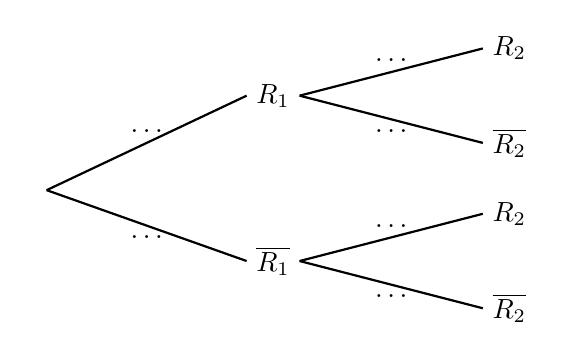
\begin{tikzpicture}[xscale=1,yscale=1]
			% Styles (MODIFIABLES)
			\tikzstyle{fleche}=[-,>=latex,thick]
			\tikzstyle{noeud}=[rounded corners=5pt]
			\tikzstyle{feuille}=[]
			\tikzstyle{commentaire}=[black]
			% Dimensions (MODIFIABLES)
			\def\DistanceInterNiveaux{3}
			\def\DistanceInterFeuilles{1.2}
			% Dimensions calculées (NON MODIFIABLES)
			\def\NiveauA{(0)*\DistanceInterNiveaux}
			\def\NiveauB{(1.0)*\DistanceInterNiveaux}
			\def\NiveauC{(2.0)*\DistanceInterNiveaux}
			\def\NiveauD{(2.750)*\DistanceInterNiveaux}
			\def\NiveauE{(3.5)*\DistanceInterNiveaux}
			\def\InterFeuilles{(-1)*\DistanceInterFeuilles}
			% Noeuds (MODIFIABLES : Styles et Coefficients d'InterFeuilles)
			%	\node[commentaire] (epreuve1) at ({\NiveauB},{(0)*\InterFeuilles}) {\scriptsize Observation};
			%	\node[commentaire] (epreuve2) at ({\NiveauC},{(0)*\InterFeuilles}) {\scriptsize Cause}; 
			%	\node[commentaire] (issues) at ({\NiveauD},{(0)*\InterFeuilles}) {\scriptsize Issues};
			%	\node[commentaire] (probas) at ({\NiveauE},{(0)*\InterFeuilles}) {\scriptsize Probabilités};
			% 
			\node[noeud] (R) at ({\NiveauA},{(2.00)*\InterFeuilles}) {};
			\node[noeud] (Ra) at ({\NiveauB},{(1)*\InterFeuilles}) {$R_1$};
			\node[feuille] (Raa) at ({\NiveauC},{(0.5)*\InterFeuilles}) {$R_2$}; 
			\node[feuille] (Rab) at ({\NiveauC},{(1.5)*\InterFeuilles}) {$\overline{R_2}$}; 
			\node[noeud] (Rb) at ({\NiveauB},{(2.75)*\InterFeuilles}) {$\overline{R_1}$};
			\node[feuille] (Rba) at ({\NiveauC},{(2.25)*\InterFeuilles}) {$R_2$}; 
			\node[feuille] (Rbb) at ({\NiveauC},{(3.25)*\InterFeuilles}) {$\overline{R_2}$}; 
			%
			%	\node[commentaire] (I1) at ({\NiveauD},{(0.5)*\InterFeuilles}) {$A\cap B$}; 
			%	\node[commentaire] (I2) at ({\NiveauD},{(1.5)*\InterFeuilles}) {$A\cap \overline{B}$}; 
			%	\node[commentaire] (I3) at ({\NiveauD},{(2.25)*\InterFeuilles}) {$\overline{A}\cap B$}; 
			%	\node[commentaire] (I4) at ({\NiveauD},{(3.25)*\InterFeuilles}) {$\overline{A}\cap \overline{B}$};
			%	%
			%	\node[commentaire] (P1) at ({\NiveauE},{(0.5)*\InterFeuilles}) {$P(A\cap B)= $}; 
			%	\node[commentaire] (P2) at ({\NiveauE},{(1.5)*\InterFeuilles}){$P(A\cap \overline{B})= $}; 
			%	%	\draw (P2.east) node[anchor=west, commentaire] {Faux négatif};
			%	\node[commentaire] (P3) at ({\NiveauE},{(2.25)*\InterFeuilles}){$P(\overline{A}\cap B)= $}; 
			%	%	\draw (P3.east) node[anchor=west, commentaire] {Faux positif};
			%	\node[commentaire] (P4) at ({\NiveauE},{(3.25)*\InterFeuilles}) {$P(\overline{A}\cap \overline{B})=$}; 
			%	%		\draw[ ultra thick] ({\NiveauE-1},{(3.55)*\InterFeuilles}) -- ({\NiveauE+1},{(3.55)*\InterFeuilles}) ;
			%	%		\node[commentaire] (P5) at ({\NiveauE},{(3.75)*\InterFeuilles})  {\textbf{Total}$=\ldots $}; 
			%	
			% Arcs (MODIFIABLES : Styles)
			\draw[fleche] (R.east)--(Ra.west) node[midway, above]{$\ldots$};
			\draw[fleche] (Ra.east)--(Raa.west) node[midway, above]{$\ldots$};
			\draw[fleche] (Ra.east)--(Rab.west) node[midway, below]{$\ldots$};
			\draw[fleche] (R.east)--(Rb.west) node[midway, below]{$\ldots$};
			\draw[fleche] (Rb.east)--(Rba.west) node[midway, above]{$\ldots$};
			\draw[fleche] (Rb.east)--(Rbb.west) node[midway, below]{$\ldots$};
		\end{tikzpicture} 
	}
	\hfill 
	\parbox{0.6\linewidth}{
		Soit les événements $R_1$   \og la boule tirée au premier est rouge\fg  et $R_2$   \og la boule tirée au second tour est rouge\fg.    
		\begin{enumerate}[leftmargin=*, label=\arabic*)]
			\item Complétez l'arbre de probabilité qui modélise cette expérience aléatoire.
			\item Quelle est la probabilité qu'une boule rouge soit tirée au deuxième tirage ?
		\end{enumerate}	
	}
\end{exercise}
\begin{exercise}[tirage sans remise] \hfill   \\  
	\parbox{0.38\linewidth}{
		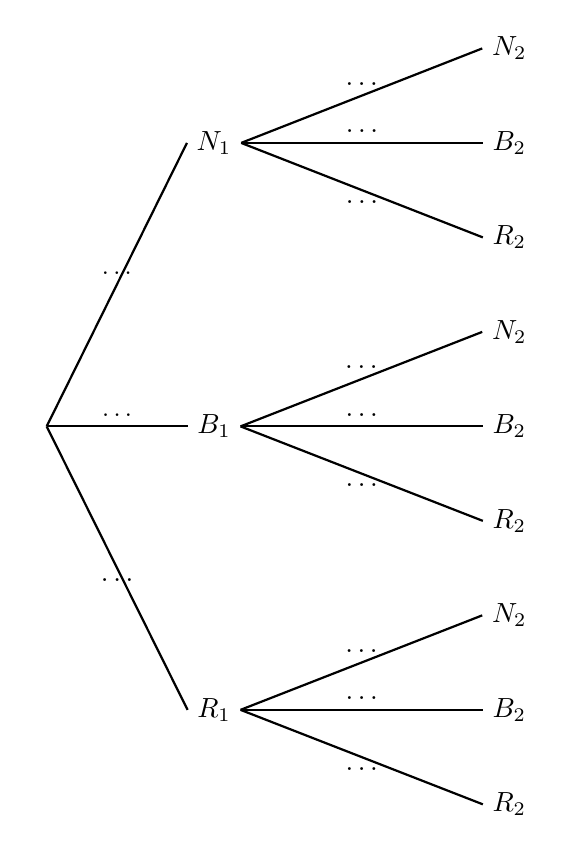
\begin{tikzpicture}[xscale=1,yscale=1]
			% Styles (MODIFIABLES)
			\tikzstyle{fleche}=[-,>=latex,thick]
			\tikzstyle{noeud}=[rounded corners=5pt]
			\tikzstyle{feuille}=[]
			\tikzstyle{commentaire}=[black]
			% Dimensions (MODIFIABLES)
			\def\DistanceInterNiveaux{3}
			\def\DistanceInterFeuilles{1.2}
			% Dimensions calculées (NON MODIFIABLES)
			\def\NiveauA{(0)*\DistanceInterNiveaux}
			\def\NiveauB{(0.75)*\DistanceInterNiveaux}
			\def\NiveauC{(2.0)*\DistanceInterNiveaux}
			\def\NiveauD{(2.750)*\DistanceInterNiveaux}
			\def\NiveauE{(3.5)*\DistanceInterNiveaux}
			\def\InterFeuilles{(-1)*\DistanceInterFeuilles}
			% Noeuds (MODIFIABLES : Styles et Coefficients d'InterFeuilles)
			%	\node[commentaire] (epreuve1) at ({\NiveauB},{(0)*\InterFeuilles}) {\scriptsize Observation};
			%	\node[commentaire] (epreuve2) at ({\NiveauC},{(0)*\InterFeuilles}) {\scriptsize Cause}; 
			%	\node[commentaire] (issues) at ({\NiveauD},{(0)*\InterFeuilles}) {\scriptsize Issues};
			%	\node[commentaire] (probas) at ({\NiveauE},{(0)*\InterFeuilles}) {\scriptsize Probabilités};
			% 
			\node[noeud] (R) at ({\NiveauA},{(5)*\InterFeuilles}) {};
			\node[noeud] (Ra) at ({\NiveauB},{(2)*\InterFeuilles}) {$N_1$};
			\node[feuille] (Raa) at ({\NiveauC},{(1)*\InterFeuilles}) {$N_2$}; 
			\node[feuille] (Rab) at ({\NiveauC},{(2)*\InterFeuilles}) {$B_2$}; 
			\node[feuille] (Rac) at ({\NiveauC},{(3)*\InterFeuilles}) {$R_2$}; 
			\node[noeud] (Rb) at ({\NiveauB},{(5)*\InterFeuilles}) {$B_1$};
			\node[feuille] (Rba) at ({\NiveauC},{(4)*\InterFeuilles}) {$N_2$}; 
			\node[feuille] (Rbb) at ({\NiveauC},{(5)*\InterFeuilles}) {$B_2$};
			\node[feuille] (Rbc) at ({\NiveauC},{(6)*\InterFeuilles}) {$R_2$}; 
			\node[noeud] (Rc) at ({\NiveauB},{(8)*\InterFeuilles}) {$R_1$};
			\node[feuille] (Rca) at ({\NiveauC},{(7)*\InterFeuilles}) {$N_2$}; 
			\node[feuille] (Rcb) at ({\NiveauC},{(8)*\InterFeuilles}) {$B_2$}; 
			\node[feuille] (Rcc) at ({\NiveauC},{(9)*\InterFeuilles}) {$R_2$}; 
			%
			%	\node[commentaire] (I1) at ({\NiveauD},{(0.5)*\InterFeuilles}) {$A\cap B$}; 
			%	\node[commentaire] (I2) at ({\NiveauD},{(1.5)*\InterFeuilles}) {$A\cap \overline{B}$}; 
			%	\node[commentaire] (I3) at ({\NiveauD},{(2.25)*\InterFeuilles}) {$\overline{A}\cap B$}; 
			%	\node[commentaire] (I4) at ({\NiveauD},{(3.25)*\InterFeuilles}) {$\overline{A}\cap \overline{B}$};
			%	%
			%	\node[commentaire] (P1) at ({\NiveauE},{(0.5)*\InterFeuilles}) {$P(A\cap B)= $}; 
			%	\node[commentaire] (P2) at ({\NiveauE},{(1.5)*\InterFeuilles}){$P(A\cap \overline{B})= $}; 
			%	%	\draw (P2.east) node[anchor=west, commentaire] {Faux négatif};
			%	\node[commentaire] (P3) at ({\NiveauE},{(2.25)*\InterFeuilles}){$P(\overline{A}\cap B)= $}; 
			%	%	\draw (P3.east) node[anchor=west, commentaire] {Faux positif};
			%	\node[commentaire] (P4) at ({\NiveauE},{(3.25)*\InterFeuilles}) {$P(\overline{A}\cap \overline{B})=$}; 
			%	%		\draw[ ultra thick] ({\NiveauE-1},{(3.55)*\InterFeuilles}) -- ({\NiveauE+1},{(3.55)*\InterFeuilles}) ;
			%	%		\node[commentaire] (P5) at ({\NiveauE},{(3.75)*\InterFeuilles})  {\textbf{Total}$=\ldots $}; 
			%	
			% Arcs (MODIFIABLES : Styles)
			\draw[fleche] (R.east)--(Ra.west) node[midway, above]{\small$\ldots$};
			\draw[fleche] (Ra.east)--(Raa.west) node[midway, above]{$\ldots$};
			\draw[fleche] (Ra.east)--(Rab.west) node[midway, above]{$\ldots$};
			\draw[fleche] (Ra.east)--(Rac.west) node[midway, below]{$\ldots$};
			\draw[fleche] (R.east)--(Rb.west) node[midway, above]{\small$\ldots$};
			\draw[fleche] (Rb.east)--(Rba.west) node[midway, above]{$\ldots$};
			\draw[fleche] (Rb.east)--(Rbb.west) node[midway, above]{$\ldots$};
			\draw[fleche] (Rb.east)--(Rbc.west) node[midway, below]{$\ldots$};
			\draw[fleche] (R.east)--(Rc.west) node[midway, below]{$\ldots$};
			\draw[fleche] (Rc.east)--(Rca.west) node[midway, above]{$\ldots$};
			\draw[fleche] (Rc.east)--(Rcb.west) node[midway, above]{$\ldots$};
			\draw[fleche] (Rc.east)--(Rcc.west) node[midway, below]{$\ldots$};
		\end{tikzpicture} 
	}
	\hfill 
	\parbox{0.6\linewidth}{Une urne opaque contient 20 boules indiscernables au toucher : 8 Noires, 7 Blanches et 5 Rouges.  	On tire au hasard une boule de l'urne, on note sa couleur sans la remettre, puis on tire de nouveau une boule de l'urne et on note sa couleur.\\
		Soit les événements $N_1$, $B_1$ et $R_1$ les événements correspondant à tirer une noir , une blanche et une boule rouge au premier tirage. De même les événements $N_2$, $B_2$ et $R_2$ correspondent aux résultats du second tirage.
		\begin{enumerate}[leftmargin=*, label=\arabic*)]
			\item Complétez l'arbre de probabilité qui modélise cette expérience aléatoire.
			\item Quelle est la probabilité de tirer deux boules noires ?
			\item En déduire la probabilité de tirer une boule Blanche puis une boule Rouge ?
			\item Quelle est la probabilité de tirer une boule Blanche et une boule Rouge ?  
			\item Quelle est la probabilité qu'une boule rouge soit tirée au deuxième tirage ?
		\end{enumerate}	
	}
\end{exercise}
\begin{exercise}\hfill \\
	On dispose de deux urnes, A et B. L'urne $A$ contient une boule rouge et trois vertes, et l'urne $B$ contient 3 boules rouges et une verte. On lance un dé cubique équilibré pour choisir une urne : s'il tombe sur le 6, on tire une boule de l'urne $A$, sinon de l'urne $B$.\\
	\parbox{0.38\linewidth}{
		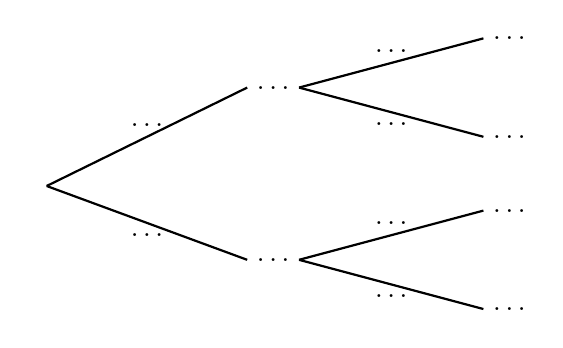
\begin{tikzpicture}[xscale=1,yscale=1]
			% Styles (MODIFIABLES)
			\tikzstyle{fleche}=[-,>=latex,thick]
			\tikzstyle{noeud}=[rounded corners=5pt]
			\tikzstyle{feuille}=[]
			\tikzstyle{commentaire}=[black]
			% Dimensions (MODIFIABLES)
			\def\DistanceInterNiveaux{3}
			\def\DistanceInterFeuilles{1.25}
			% Dimensions calculées (NON MODIFIABLES)
			\def\NiveauA{(0)*\DistanceInterNiveaux}
			\def\NiveauB{(1.0)*\DistanceInterNiveaux}
			\def\NiveauC{(2.0)*\DistanceInterNiveaux}
			\def\NiveauD{(2.750)*\DistanceInterNiveaux}
			\def\NiveauE{(3.5)*\DistanceInterNiveaux}
			\def\InterFeuilles{(-1)*\DistanceInterFeuilles}
			% Noeuds (MODIFIABLES : Styles et Coefficients d'InterFeuilles)
			%	\node[commentaire] (epreuve1) at ({\NiveauB},{(0)*\InterFeuilles}) {\scriptsize Observation};
			%	\node[commentaire] (epreuve2) at ({\NiveauC},{(0)*\InterFeuilles}) {\scriptsize Cause}; 
			%	\node[commentaire] (issues) at ({\NiveauD},{(0)*\InterFeuilles}) {\scriptsize Issues};
			%	\node[commentaire] (probas) at ({\NiveauE},{(0)*\InterFeuilles}) {\scriptsize Probabilités};
			% 
			\node[noeud] (R) at ({\NiveauA},{(2.00)*\InterFeuilles}) {};
			\node[noeud] (Ra) at ({\NiveauB},{(1)*\InterFeuilles}) {$\ldots$};
			\node[feuille] (Raa) at ({\NiveauC},{(0.5)*\InterFeuilles}) {$\ldots$}; 
			\node[feuille] (Rab) at ({\NiveauC},{(1.5)*\InterFeuilles}) {${\ldots}$}; 
			\node[noeud] (Rb) at ({\NiveauB},{(2.75)*\InterFeuilles}) {${\ldots}$};
			\node[feuille] (Rba) at ({\NiveauC},{(2.25)*\InterFeuilles}) {$\ldots$}; 
			\node[feuille] (Rbb) at ({\NiveauC},{(3.25)*\InterFeuilles}) {$ {\ldots}$}; 
			%
			%	\node[commentaire] (I1) at ({\NiveauD},{(0.5)*\InterFeuilles}) {$A\cap B$}; 
			%	\node[commentaire] (I2) at ({\NiveauD},{(1.5)*\InterFeuilles}) {$A\cap \overline{B}$}; 
			%	\node[commentaire] (I3) at ({\NiveauD},{(2.25)*\InterFeuilles}) {$\overline{A}\cap B$}; 
			%	\node[commentaire] (I4) at ({\NiveauD},{(3.25)*\InterFeuilles}) {$\overline{A}\cap \overline{B}$};
			%	%
			%	\node[commentaire] (P1) at ({\NiveauE},{(0.5)*\InterFeuilles}) {$P(A\cap B)= $}; 
			%	\node[commentaire] (P2) at ({\NiveauE},{(1.5)*\InterFeuilles}){$P(A\cap \overline{B})= $}; 
			%	%	\draw (P2.east) node[anchor=west, commentaire] {Faux négatif};
			%	\node[commentaire] (P3) at ({\NiveauE},{(2.25)*\InterFeuilles}){$P(\overline{A}\cap B)= $}; 
			%	%	\draw (P3.east) node[anchor=west, commentaire] {Faux positif};
			%	\node[commentaire] (P4) at ({\NiveauE},{(3.25)*\InterFeuilles}) {$P(\overline{A}\cap \overline{B})=$}; 
			%	%		\draw[ ultra thick] ({\NiveauE-1},{(3.55)*\InterFeuilles}) -- ({\NiveauE+1},{(3.55)*\InterFeuilles}) ;
			%	%		\node[commentaire] (P5) at ({\NiveauE},{(3.75)*\InterFeuilles})  {\textbf{Total}$=\ldots $}; 
			%	
			% Arcs (MODIFIABLES : Styles)
			\draw[fleche] (R.east)--(Ra.west) node[midway, above]{$\ldots$};
			\draw[fleche] (Ra.east)--(Raa.west) node[midway, above]{$\ldots$};
			\draw[fleche] (Ra.east)--(Rab.west) node[midway, below]{$\ldots$};
			\draw[fleche] (R.east)--(Rb.west) node[midway, below]{$\ldots$};
			\draw[fleche] (Rb.east)--(Rba.west) node[midway, above]{$\ldots$};
			\draw[fleche] (Rb.east)--(Rbb.west) node[midway, below]{$\ldots$};
		\end{tikzpicture} 
	}
	\hfill 
	\parbox{0.6\linewidth}{
		Soit les événements $D$ \og le dé tombe sur $6$\fg, $R$   \og la boule tirée au premier est rouge\fg  et $V$   \og la boule tirée au second tour est verte\fg.    
		\begin{enumerate}[leftmargin=*, label=\arabic*)]
			\item Complétez l'arbre de probabilité qui modélise cette expérience aléatoire.
			\item Quelle est la probabilité qu'une boule verte soit tirée.
		\end{enumerate}	
	}
\end{exercise}
\begin{exercise} \hfill  \smallskip\\
	\parbox{0.74\linewidth}{
		On dispose de 3 urnes, $A$, $B$ et $C$.
		\begin{enumerate}[leftmargin=*, label=\textbullet]
			\item	L'urne $A$ contient 11 boules rouges et 6 vertes
			\item 	L'urne $B$ contient 10 boules rouges et 3 vertes
			\item	L'urne $C$ contient 3 boules rouges et 6 vertes
		\end{enumerate} 	
		On lance un dé cubique équilibré pour choisir une urne : s'il tombe sur un nombre inférieur ou égal à 4, on tire une boule de l'urne $A$, s'il tombe sur $6$ de l'urne $B$, et sur les autres cas il tire  de l'urne $C$. 
		\begin{enumerate}[leftmargin=*, label=\arabic*)]
			\item Complétez l'arbre de probabilité qui modélise cette expérience aléatoire.
			\item Quelle est la probabilité qu'une boule tirée soit rouge ?
			\item On sait qu'on a tiré une boulle rouge, quelle est la probabilité que la boule provient de l'urne $C$ ?
		\end{enumerate}	
	}\; 
	\parbox{0.25\linewidth}{
		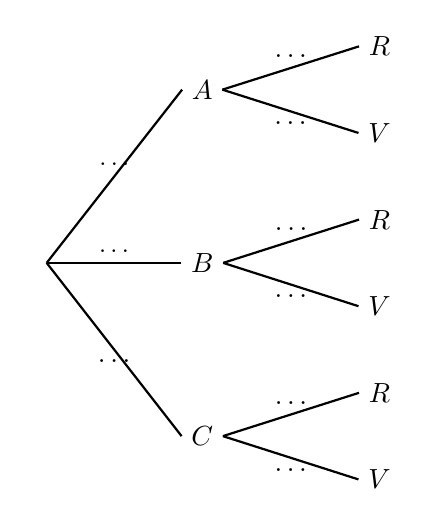
\begin{tikzpicture}[xscale=1,yscale=1]
			% Styles (MODIFIABLES)
			\tikzstyle{fleche}=[-,>=latex,thick]
			\tikzstyle{noeud}=[rounded corners=5pt]
			\tikzstyle{feuille}=[]
			\tikzstyle{commentaire}=[black]
			% Dimensions (MODIFIABLES)
			\def\DistanceInterNiveaux{3}
			\def\DistanceInterFeuilles{1.1}
			% Dimensions calculées (NON MODIFIABLES)
			\def\NiveauA{(0)*\DistanceInterNiveaux}
			\def\NiveauB{(0.70)*\DistanceInterNiveaux}
			\def\NiveauC{(1.45)*\DistanceInterNiveaux}
			\def\NiveauD{(2.750)*\DistanceInterNiveaux}
			\def\NiveauE{(3.5)*\DistanceInterNiveaux}
			\def\InterFeuilles{(-1)*\DistanceInterFeuilles}
			% Noeuds (MODIFIABLES : Styles et Coefficients d'InterFeuilles)
			%	\node[commentaire] (epreuve1) at ({\NiveauB},{(0)*\InterFeuilles}) {\scriptsize Observation};
			%	\node[commentaire] (epreuve2) at ({\NiveauC},{(0)*\InterFeuilles}) {\scriptsize Cause}; 
			%	\node[commentaire] (issues) at ({\NiveauD},{(0)*\InterFeuilles}) {\scriptsize Issues};
			%	\node[commentaire] (probas) at ({\NiveauE},{(0)*\InterFeuilles}) {\scriptsize Probabilités};
			% 
			\node[noeud] (R) at ({\NiveauA},{(3.5)*\InterFeuilles}) {};
			\node[noeud] (Ra) at ({\NiveauB},{(1.5)*\InterFeuilles}) {$A$};
			\node[feuille] (Raa) at ({\NiveauC},{(1)*\InterFeuilles}) {$R$}; 
			\node[feuille] (Rab) at ({\NiveauC},{(2)*\InterFeuilles}) {${V}$}; 
			\node[noeud] (Rb) at ({\NiveauB},{(3.5)*\InterFeuilles}) {${B}$};
			\node[feuille] (Rba) at ({\NiveauC},{(3)*\InterFeuilles}) {$R$}; 
			\node[feuille] (Rbb) at ({\NiveauC},{(4)*\InterFeuilles}) {${V}$}; 
			\node[noeud] (Rc) at ({\NiveauB},{(5.5)*\InterFeuilles}) {${C}$};
			\node[feuille] (Rca) at ({\NiveauC},{(5)*\InterFeuilles}) {$R$}; 
			\node[feuille] (Rcb) at ({\NiveauC},{(6)*\InterFeuilles}) {${V}$}; 
			%
			%	\node[commentaire] (I1) at ({\NiveauD},{(0.5)*\InterFeuilles}) {$A\cap B$}; 
			%	\node[commentaire] (I2) at ({\NiveauD},{(1.5)*\InterFeuilles}) {$A\cap \overline{B}$}; 
			%	\node[commentaire] (I3) at ({\NiveauD},{(2.25)*\InterFeuilles}) {$\overline{A}\cap B$}; 
			%	\node[commentaire] (I4) at ({\NiveauD},{(3.25)*\InterFeuilles}) {$\overline{A}\cap \overline{B}$};
			%	%
			%	\node[commentaire] (P1) at ({\NiveauE},{(0.5)*\InterFeuilles}) {$P(A\cap B)= $}; 
			%	\node[commentaire] (P2) at ({\NiveauE},{(1.5)*\InterFeuilles}){$P(A\cap \overline{B})= $}; 
			%	%	\draw (P2.east) node[anchor=west, commentaire] {Faux négatif};
			%	\node[commentaire] (P3) at ({\NiveauE},{(2.25)*\InterFeuilles}){$P(\overline{A}\cap B)= $}; 
			%	%	\draw (P3.east) node[anchor=west, commentaire] {Faux positif};
			%	\node[commentaire] (P4) at ({\NiveauE},{(3.25)*\InterFeuilles}) {$P(\overline{A}\cap \overline{B})=$}; 
			%	%		\draw[ ultra thick] ({\NiveauE-1},{(3.55)*\InterFeuilles}) -- ({\NiveauE+1},{(3.55)*\InterFeuilles}) ;
			%	%		\node[commentaire] (P5) at ({\NiveauE},{(3.75)*\InterFeuilles})  {\textbf{Total}$=\ldots $}; 
			%	
			% Arcs (MODIFIABLES : Styles)
			\draw[fleche] (R.east)--(Ra.west) node[midway, above]{\small$\ldots$};
			\draw[fleche] (Ra.east)--(Raa.west) node[midway, above]{$\ldots$};
			\draw[fleche] (Ra.east)--(Rab.west) node[midway, below]{$\ldots$};
			\draw[fleche] (R.east)--(Rb.west) node[midway, above]{\small$\ldots$};
			\draw[fleche] (Rb.east)--(Rba.west) node[midway, above]{$\ldots$};
			\draw[fleche] (Rb.east)--(Rbb.west) node[midway, below]{$\ldots$};
			\draw[fleche] (R.east)--(Rc.west) node[midway, below]{$\ldots$};
			\draw[fleche] (Rc.east)--(Rca.west) node[midway, above]{$\ldots$};
			\draw[fleche] (Rc.east)--(Rcb.west) node[midway, below]{$\ldots$};
		\end{tikzpicture} 
	}
\end{exercise}

%----------------------------------------------------------------------------------------

\newpage 







%----------------------------------------------------------------------------------------
%	 
%----------------------------------------------------------------------------------------

\newpage 
\loadgeometry{marginlayout}  
\pagestyle{scrheadings} % Print headers again  
\KOMAoptions{
	headwidth=textwithmarginpar,
	headsepline=true,
	headsepline= 0.5pt,
	footwidth=textwithmarginpar,
} 
\onehalfspacing
\section{Événements indépendants, applications}



\begin{theorem}[Théorème de Bayes] Pour deux événements $A$ et $B$ (avec $P\left(A\right)$ et $P(B)  \neq 0$), on a :
	\setlength{\abovedisplayskip}{3pt}
	\setlength{\belowdisplayskip}{3pt}
	$$
	P(A\cap B)= P(A)P_A(B)=P(B)P_B(A)
	$$
\end{theorem}
\marginnote{
	\begin{tBox}[leftline=false]
		On peut désormais dire que $A$ et $B$ sont indépendants.
	\end{tBox}
}  
\begin{corollary} Pour deux événements $A$ et $B$ de probabilité non nulle. Les affirmations suivantes sont équivalentes :
	
	\begin{enumerate}[label={(\alph*)}]
		\item $B$ est indépendant de $A$ ($P_A(B)=P(B)$)
		\item $A$ est indépendant de $B$ ($P_B(A)=P(A)$)
		\item $P(A\cap B) =P(A)\times P(B)$
	\end{enumerate} 
\end{corollary}
\begin{proof}$(a\Rightarrow c)$ : Si $P_A(B)=P(B)$ alors d'après Bayes $P(A\cap B)=P(A)P_A(B)= P(A)P(B)$.\\ 
	$(c\Rightarrow (a)$ :
	Si  $P(A\cap B) =P(A)\times P(B)$ alors $P_A(B)=\tfrac{P(A\cap B)}{P(A)}=\tfrac{P(A)P(B)}{P(A)}=P(B)$.
\end{proof}
\begin{remark} Pour simplifier on considère que deux événments sont indépendants si $P(A\cap B)=P(A)P(B)$ même si leur probabilités sont nulles.
\end{remark}
\begin{theorem} $A^*$ est égal à $A$ ou à $\overline{A}$, $B^*$ est égal à $B$ ou à $\overline{B}$.
	
	Si les événements $A$ et $B$ sont indépendants, alors $A^*$ et $B^*$ sont aussi indépendants.
	
	En particulier $P_A(B)=P_{\overline{A}}(B)=P(B)$.
\end{theorem}
\begin{proof} Si $A$ et $B$ sont indépendants. Nous allons montrer que $\overline{A}$ et $B$ sont indépendants.
	
	$\begin{WithArrows}
		P(\overline{A}\cap B)& = P(B) - P(A\cap B) \Arrow{$A$ et $B$ indépendants}\\
		& = P(B) - P(A)P(B)\\
		&= P(B) (1-P(A))\\
		&= P(\overline{A})P(B)	
	\end{WithArrows}
	$
\end{proof}

%----------------------------------------------------------------------------------------
%	EXERCICES
%----------------------------------------------------------------------------------------

\newpage 
\loadgeometry{widelayout}  
\pagestyle{scrheadings} % Print headers again  
\KOMAoptions{
	headwidth=textwithmarginpar,
	headsepline=true,
	headsepline= 0.5pt,
	footwidth=textwithmarginpar,
} 
\onehalfspacing
\subsection{Exercices : Indépendance de deux événements. Application}

\begin{exercise} Cochez si les événements $A$ et $B$ sont indépendants ou non.
	
	\noindent\QCM[VF,Alterne,Stretch=1.0,NomV=Indépendants,NomF={\small Non indépendants},  Largeur=3.0cm]{% 
		{
			$P(A)=\tfrac{7}{8}$, $P(B)=\tfrac{2}{7}$ et $P(A\cap B)=\tfrac{1}{4}$.}&1,% 
		{ $P(A)=0,2$, $P(B)=0,8$ et $P(A \cap B)=0,9$.}&2,% 
		{$P(A)=0,48$, $P(B)=0,25$.  $A$ et $B$ sont incompatibles.}&2,% 
		{$P(A)=0,4$, $P(B)=0,8$ et $P(A \cap B)=0,32$.}&1,%  
	} 
\end{exercise} \smallskip
\begin{exercise}\hfill \\ Les événements $A$ et $B$ sont indépendants, calculez les probabilités demandées dans chaque cas.
	\begin{enumerate}[leftmargin=*,label=\arabic*)]
		\item $P(A)=0,8$ et $P(A \cap B)=0,45$. Calculer $P(B)$.
		\item $P(A)=P(B)$ et $P(A \cap B)=0,25$. Calculer $P(A)$
		\item $P(\overline{A})=0,6$ et $P(A \cap B)=0,3$. Calculer $P(A)$ puis $P(B)$.
		\item $P(A)=0.5$ et $P(B)=0.7$, calculer $P(A\cap B)$ et $P(\overline{A} \cap B)$
	\end{enumerate} 
\end{exercise}

\begin{exercise}  \hfill \\
	$P(X)=0.5$, $P(Y)=0.3$ et $P(X\cup Y)=0.95$. Montrer que $X$ et $Y$ sont indépendants.
\end{exercise}
\begin{exercise} \hfill \\
	$P(X)=0.3$, $P(Y)=0.42$ et $P(X\cup Y)=0.594$. Montrer que $X$ et $Y$ sont indépendants.
\end{exercise}
\begin{exercise} \hfill \\
	On lance un dé cubique équilibré. Soit les événements $A=$  \og le résultat est $\geqslant 4$ \fg{} et $B=$ \og le résultat est un nombre pair \fg{}. Les événements $A$ et $B$ sont-ils indépendants ?
\end{exercise}\smallskip
\begin{exercise} \hfill \\
	On rappelle que, dans un jeu de 32 cartes, on trouve quatre couleurs (Carreau $\diamondsuit$ et Coeur $\heartsuit$ sont de couleur rouge. Trèfle $\clubsuit$ et Pique $\spadesuit$) et, dans chaque couleur, on a une série de 8 cartes (7, 8, 9, 10, Valet, Dame, Roi, As). \\
	On tire au hasard une carte d'un jeu de 32~cartes. Soit les événements   $A=$ \og la carte tirée est un roi \fg,  $B=$ \og la carte tirée est un as\fg  et  $C=$ \og la carte tirée est rouge\fg   
	\begin{enumerate}[label=\arabic*),leftmargin=*]
		\item Justifiez que les événements $A$ et $C$ sont indépendants.
		\item Justifiez que les événements $A$ et $\overline{B}$ ne sont pas indépendants.
		\item Les événements $A\cup C$ et $B$ sont-ils indépendants ?
	\end{enumerate}
\end{exercise}
\begin{exercise} \hfill \\
	Les élèves d'un collège doivent choisir une option parmi \og latin \fg{} et  \og théâtre \fg{} et une langue vivantes parmi \og allemand \fg{} et \og italien \fg{}. Le tableau ci-dessous donne la répartition des élèves.\smallskip\\
	\noindent\parbox{0.6\linewidth}{ 
		\begin{enumerate}[leftmargin=*,label=\arabic*)]
			\item Les événements \og faire du théâtre et de l'italien \fg{} et \og faire du théâtre \fg{} sont-ils indépendants ? 
			\item Les événements \og faire du latin \fg{} et \og faire de l'allemand \fg{} sont-ils indépendants ? 
			\item Les événements \og faire du latin \fg{} et \og faire du théâtre \fg{} sont-ils indépendants ? 
		\end{enumerate}
	}\hfill 
	\parbox{0.38\linewidth}{ 
		%		\renewcommand{\arraystretch}{1.6}
		\begin{tabular}{|c|c|c|c|}
			\cline{2-4} \multicolumn{1}{c|}{} & Italien & Allemand & Total \\\hline
			Latin & $30$ & $120$ & $150$ \\\hline 
			Théâtre & $90$ & $80$ & $170$ \\\hline 
			Total & $120$ & $200$ & $320$ \\\hline 
		\end{tabular}
	}  \smallskip
\end{exercise}
\begin{exercise}[tirage avec remise]\hfill \\
	Une urne opaque contient 11 boules rouges et 12 boules vertes indiscernables au toucher. 	On tire au hasard une boule de l'urne, on note sa couleur avant de la remettre, puis on tire de nouveau une boule de l'urne et on note sa couleur.  \\  
	\parbox{0.38\linewidth}{
		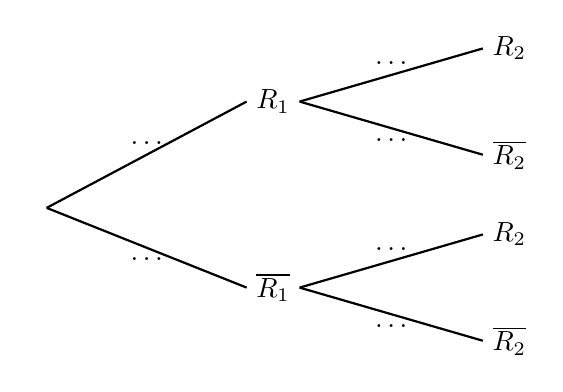
\begin{tikzpicture}[xscale=1,yscale=1]
			% Styles (MODIFIABLES)
			\tikzstyle{fleche}=[-,>=latex,thick]
			\tikzstyle{noeud}=[rounded corners=5pt]
			\tikzstyle{feuille}=[]
			\tikzstyle{commentaire}=[black]
			% Dimensions (MODIFIABLES)
			\def\DistanceInterNiveaux{3}
			\def\DistanceInterFeuilles{1.35}
			% Dimensions calculées (NON MODIFIABLES)
			\def\NiveauA{(0)*\DistanceInterNiveaux}
			\def\NiveauB{(1.0)*\DistanceInterNiveaux}
			\def\NiveauC{(2.0)*\DistanceInterNiveaux}
			\def\NiveauD{(2.750)*\DistanceInterNiveaux}
			\def\NiveauE{(3.5)*\DistanceInterNiveaux}
			\def\InterFeuilles{(-1)*\DistanceInterFeuilles}
			% Noeuds (MODIFIABLES : Styles et Coefficients d'InterFeuilles)
			%	\node[commentaire] (epreuve1) at ({\NiveauB},{(0)*\InterFeuilles}) {\scriptsize Observation};
			%	\node[commentaire] (epreuve2) at ({\NiveauC},{(0)*\InterFeuilles}) {\scriptsize Cause}; 
			%	\node[commentaire] (issues) at ({\NiveauD},{(0)*\InterFeuilles}) {\scriptsize Issues};
			%	\node[commentaire] (probas) at ({\NiveauE},{(0)*\InterFeuilles}) {\scriptsize Probabilités};
			% 
			\node[noeud] (R) at ({\NiveauA},{(2.00)*\InterFeuilles}) {};
			\node[noeud] (Ra) at ({\NiveauB},{(1)*\InterFeuilles}) {$R_1$};
			\node[feuille] (Raa) at ({\NiveauC},{(0.5)*\InterFeuilles}) {$R_2$}; 
			\node[feuille] (Rab) at ({\NiveauC},{(1.5)*\InterFeuilles}) {$\overline{R_2}$}; 
			\node[noeud] (Rb) at ({\NiveauB},{(2.75)*\InterFeuilles}) {$\overline{R_1}$};
			\node[feuille] (Rba) at ({\NiveauC},{(2.25)*\InterFeuilles}) {$R_2$}; 
			\node[feuille] (Rbb) at ({\NiveauC},{(3.25)*\InterFeuilles}) {$\overline{R_2}$}; 
			%
			%	\node[commentaire] (I1) at ({\NiveauD},{(0.5)*\InterFeuilles}) {$A\cap B$}; 
			%	\node[commentaire] (I2) at ({\NiveauD},{(1.5)*\InterFeuilles}) {$A\cap \overline{B}$}; 
			%	\node[commentaire] (I3) at ({\NiveauD},{(2.25)*\InterFeuilles}) {$\overline{A}\cap B$}; 
			%	\node[commentaire] (I4) at ({\NiveauD},{(3.25)*\InterFeuilles}) {$\overline{A}\cap \overline{B}$};
			%	%
			%	\node[commentaire] (P1) at ({\NiveauE},{(0.5)*\InterFeuilles}) {$P(A\cap B)= $}; 
			%	\node[commentaire] (P2) at ({\NiveauE},{(1.5)*\InterFeuilles}){$P(A\cap \overline{B})= $}; 
			%	%	\draw (P2.east) node[anchor=west, commentaire] {Faux négatif};
			%	\node[commentaire] (P3) at ({\NiveauE},{(2.25)*\InterFeuilles}){$P(\overline{A}\cap B)= $}; 
			%	%	\draw (P3.east) node[anchor=west, commentaire] {Faux positif};
			%	\node[commentaire] (P4) at ({\NiveauE},{(3.25)*\InterFeuilles}) {$P(\overline{A}\cap \overline{B})=$}; 
			%	%		\draw[ ultra thick] ({\NiveauE-1},{(3.55)*\InterFeuilles}) -- ({\NiveauE+1},{(3.55)*\InterFeuilles}) ;
			%	%		\node[commentaire] (P5) at ({\NiveauE},{(3.75)*\InterFeuilles})  {\textbf{Total}$=\ldots $}; 
			%	
			% Arcs (MODIFIABLES : Styles)
			\draw[fleche] (R.east)--(Ra.west) node[midway, above]{$\ldots$};
			\draw[fleche] (Ra.east)--(Raa.west) node[midway, above]{$\ldots$};
			\draw[fleche] (Ra.east)--(Rab.west) node[midway, below]{$\ldots$};
			\draw[fleche] (R.east)--(Rb.west) node[midway, below]{$\ldots$};
			\draw[fleche] (Rb.east)--(Rba.west) node[midway, above]{$\ldots$};
			\draw[fleche] (Rb.east)--(Rbb.west) node[midway, below]{$\ldots$};
		\end{tikzpicture} 
	}
	\hfill 
	\parbox{0.6\linewidth}{
		Soit les événements $R_1$   \og la boule tirée au premier est rouge\fg  et $R_2$   \og la boule tirée au second tour est rouge\fg.    
		\begin{enumerate}[leftmargin=*, label=\arabic*)]
			\item Complétez l'arbre de probabilité qui modélise cette expérience aléatoire.
			\item Quelle est la probabilité qu'une boule rouge soit tirée au deuxième tirage ?
			\item Justifiez que les événements $R_1$ et $R_2$ sont indépendants.
		\end{enumerate}	
	}
\end{exercise}
%---------------------------------------------------------------------------------------- 
% \newpage 
\begin{exercise}\hfill \\
	\parbox{0.6\linewidth}{
		On lance un dé cubique équilibré 2 fois consécutives. Soit l'événement $D_1=$\og obtenir un 6 au premier lancer\fg et $D_2=$ \og obtenir un 6 au second lancer\fg. 
		\begin{enumerate}[leftmargin=*, label=\arabic*)]
			\item Complétez l'arbre de probabilité qui modélise cette expérience aléatoire.
			\item Quelle est la probabilité d'obtenir deux 6 ?
			\item Montrer que les événements $\overline{D_1}$ et ${D_2}$ sont indépendants.
		\end{enumerate}	
	}
	\hfill 
	\parbox{0.38\linewidth}{
		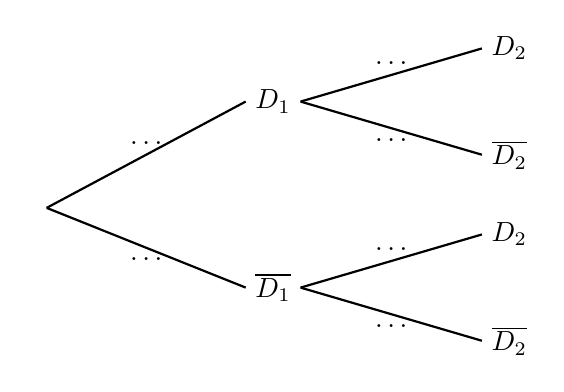
\begin{tikzpicture}[xscale=1,yscale=1]
			% Styles (MODIFIABLES)
			\tikzstyle{fleche}=[-,>=latex,thick]
			\tikzstyle{noeud}=[rounded corners=5pt]
			\tikzstyle{feuille}=[]
			\tikzstyle{commentaire}=[black]
			% Dimensions (MODIFIABLES)
			\def\DistanceInterNiveaux{3}
			\def\DistanceInterFeuilles{1.35}
			% Dimensions calculées (NON MODIFIABLES)
			\def\NiveauA{(0)*\DistanceInterNiveaux}
			\def\NiveauB{(1.0)*\DistanceInterNiveaux}
			\def\NiveauC{(2.0)*\DistanceInterNiveaux}
			\def\NiveauD{(2.750)*\DistanceInterNiveaux}
			\def\NiveauE{(3.5)*\DistanceInterNiveaux}
			\def\InterFeuilles{(-1)*\DistanceInterFeuilles}
			% Noeuds (MODIFIABLES : Styles et Coefficients d'InterFeuilles)
			%	\node[commentaire] (epreuve1) at ({\NiveauB},{(0)*\InterFeuilles}) {\scriptsize Observation};
			%	\node[commentaire] (epreuve2) at ({\NiveauC},{(0)*\InterFeuilles}) {\scriptsize Cause}; 
			%	\node[commentaire] (issues) at ({\NiveauD},{(0)*\InterFeuilles}) {\scriptsize Issues};
			%	\node[commentaire] (probas) at ({\NiveauE},{(0)*\InterFeuilles}) {\scriptsize Probabilités};
			% 
			\node[noeud] (R) at ({\NiveauA},{(2.00)*\InterFeuilles}) {};
			\node[noeud] (Ra) at ({\NiveauB},{(1)*\InterFeuilles}) {$D_1$};
			\node[feuille] (Raa) at ({\NiveauC},{(0.5)*\InterFeuilles}) {$D_2$}; 
			\node[feuille] (Rab) at ({\NiveauC},{(1.5)*\InterFeuilles}) {$\overline{D_2}$}; 
			\node[noeud] (Rb) at ({\NiveauB},{(2.75)*\InterFeuilles}) {$\overline{D_1}$};
			\node[feuille] (Rba) at ({\NiveauC},{(2.25)*\InterFeuilles}) {$D_2$}; 
			\node[feuille] (Rbb) at ({\NiveauC},{(3.25)*\InterFeuilles}) {$\overline{D_2}$}; 
			%
			%	\node[commentaire] (I1) at ({\NiveauD},{(0.5)*\InterFeuilles}) {$A\cap B$}; 
			%	\node[commentaire] (I2) at ({\NiveauD},{(1.5)*\InterFeuilles}) {$A\cap \overline{B}$}; 
			%	\node[commentaire] (I3) at ({\NiveauD},{(2.25)*\InterFeuilles}) {$\overline{A}\cap B$}; 
			%	\node[commentaire] (I4) at ({\NiveauD},{(3.25)*\InterFeuilles}) {$\overline{A}\cap \overline{B}$};
			%	%
			%	\node[commentaire] (P1) at ({\NiveauE},{(0.5)*\InterFeuilles}) {$P(A\cap B)= $}; 
			%	\node[commentaire] (P2) at ({\NiveauE},{(1.5)*\InterFeuilles}){$P(A\cap \overline{B})= $}; 
			%	%	\draw (P2.east) node[anchor=west, commentaire] {Faux négatif};
			%	\node[commentaire] (P3) at ({\NiveauE},{(2.25)*\InterFeuilles}){$P(\overline{A}\cap B)= $}; 
			%	%	\draw (P3.east) node[anchor=west, commentaire] {Faux positif};
			%	\node[commentaire] (P4) at ({\NiveauE},{(3.25)*\InterFeuilles}) {$P(\overline{A}\cap \overline{B})=$}; 
			%	%		\draw[ ultra thick] ({\NiveauE-1},{(3.55)*\InterFeuilles}) -- ({\NiveauE+1},{(3.55)*\InterFeuilles}) ;
			%	%		\node[commentaire] (P5) at ({\NiveauE},{(3.75)*\InterFeuilles})  {\textbf{Total}$=\ldots $}; 
			%	
			% Arcs (MODIFIABLES : Styles)
			\draw[fleche] (R.east)--(Ra.west) node[midway, above]{$\ldots$};
			\draw[fleche] (Ra.east)--(Raa.west) node[midway, above]{$\ldots$};
			\draw[fleche] (Ra.east)--(Rab.west) node[midway, below]{$\ldots$};
			\draw[fleche] (R.east)--(Rb.west) node[midway, below]{$\ldots$};
			\draw[fleche] (Rb.east)--(Rba.west) node[midway, above]{$\ldots$};
			\draw[fleche] (Rb.east)--(Rbb.west) node[midway, below]{$\ldots$};
		\end{tikzpicture} 
	} 
\end{exercise}

\begin{exercise}[Problème du Grand-Duc de Toscane]\hfill \\
	On lance 3 dés cubiques équilibrés ($D_1$, $D_2$ et $D_3$), et on note la face obtenue pour chaque dans l'ordre. On suppose que les résultats des lancers de chaque dé sont indépendants.
	\begin{enumerate}[leftmargin=*, label=\arabic*)]
		\item Quelle est la probabilité $P(D_2=5)$  que le second dé tombe sur $5$ ?
		\item Quelle est la probabilité $P(D_2=5 \;\text{et}\;D_3=2)$ que le second dé tombe sur $5$ et le troisième sur $2$.
		\item Quelle est la probabilité $P(D_1=2; D_2=1; D_3=3)$ que le premier dé tombe sur $2$, le second sur $1$ et le dernier sur $3$ ?
		\item Quelle est la probabilité d'obtenir simultanément un 1, un 2 et un 3 ?
		\item Identifier toutes les différentes façons d'obtenir une somme des 3 dés égale à $9$.
		\item Démontrer que la probablité d'obtenir une somme égale à $9$ est $\frac{25}{216}$.
		\item Démontrer que la probabilité d'obtenir une somme égale à $10$ est de $\frac{27}{216}$.
	\end{enumerate}
	
	
\end{exercise}


%----------------------------------------------------------------------------------------
%	EXERCICES
%----------------------------------------------------------------------------------------

\newpage 
\loadgeometry{widelayout}  
\pagestyle{scrheadings} % Print headers again  
\KOMAoptions{
	headwidth=textwithmarginpar,
	headsepline=true,
	headsepline= 0.5pt,
	footwidth=textwithmarginpar,
} 
\onehalfspacing
\section{Club maths : conditionnements paradoxaux}
%\begin{exercise}\hfill \\
%Un orchestre pratique une audition. Parmi les candidants jouant un instrument à vent, 26 des 40 hommes et 4 des 6 femmes ont été retenus. Parmi les candidats jouant un instrument à corde : 30 des 80 hommes et 19 des 49 femmes sont retenus. 
%
%On tire un candidat au hasard. Soit les événements $F=$ \og être une femme \fg, et $C=$ \og jouer un instrument à corde \fg, et $S=$ \og succés à l'audition \fg.
%	\begin{enumerate}[leftmargin=*, label=\arabic*)]
%	\item Calculer les probabilités $P_F(S)$ et  $P_{\overline{F}}(S)$.
%	\item Quel sexe semble être légérement discriminé dans ces auditions ?
%	\item Calculer les probabilités $P_{F\cap C}(S)$ et  $P_{F\cap\overline{C}}(S)$.
%	\item Calculer les probabilités $P_{\overline{F}\cap C}(S)$ et  $P_{\overline{F}\cap\overline{C}}(S)$.
%	\item Pour les musiciens jouant un instrument à corde, quel sexe semble être légérement discriminé  dans ces auditions ? Même question pour les musiciens jouant un instrument à vent.
%\end{enumerate}
%\end{exercise}
\begin{exercise}[paradoxe de Simpson] \hfill \\
	Un test clinique vise à étudier l'efficacité d'un nouveau traitement thérapeutique à des malades atteints de cancer. On choisit un participant au hasard parmi les 21100. Soit les événements 	$A  = $ \og le patient est vivant  \fg{}, $T =  $ \og le patient a suivi le traitement \fg{} et $V =  $ \og le patient réside en ville \fg{}. Les effectifs sont rassemblés dans le tableau : \\
		\begin{tabular}{|*5{c|}}
		\cline{2-5}
		\multicolumn{1}{c|}{\multirow{2}{*}{}} & \multicolumn{2}{c|}{$V$, en ville}  & \multicolumn{2}{c|}{$\overline{V}$  } \\ \cline{2-5}
		\multicolumn{1}{c|}{}   &  $T$ &  $\overline{T}$   &$T$  & $\overline{T}$   \\ \hline
		   $A$  &  1000 & 50  & 95 &  5000  \\ \hline
		  $\overline{A}$  & 9000  &  950  & 5   & 5000    \\ \hline
	\end{tabular}
	
	 
	\begin{enumerate}[leftmargin=*, label=\arabic*)]
		\item Déterminez $P_T(A)$ et $P_{\overline{T}}(A)$. 
		\item Quel semble l'effet du traitement sur les chances de survie ?
		\item Déterminez  $P_{T\cap V}(A)$, $P_{T\cap \overline{V}}(A)$.
		\item Déterminez $P_{\overline{T}\cap V}(A)$, $P_{\overline{T}\cap \overline{V}}(A)$. 
		\item Quel est l'effet du traitement  lorsqu'on prend en compte le lieu de résidence ? 
	\end{enumerate} 
\end{exercise} 
\begin{exercise}[le rouge et le noir] \hfill \\
	Trois boites contiennent chacune une carte. Une des cartes a deux faces rouges, une a deux faces noires, et la troisième une rouge et une noire. On choisit au hasard une boite, et l'on    voit que la face visible de la carte qu'elle contient est rouge. Quelle est la probabilité que l'autre soit noire ?
	% ce n'est pas 1/2, mais 1/3
\end{exercise}
\begin{exercise}[Monty Hall]
	
\end{exercise}



%----------------------------------------------------------------------------------------
%	EXERCICES
%----------------------------------------------------------------------------------------

\newpage 
\loadgeometry{widelayout}  
\pagestyle{scrheadings} % Print headers again  
\KOMAoptions{
	headwidth=textwithmarginpar,
	headsepline=true,
	headsepline= 0.5pt,
	footwidth=textwithmarginpar,
} 
\onehalfspacing

\section{Banque pour évaluation}

\begin{exercise} 
	Soit $A$ et $B$ deux événements.
	\begin{enumerate}[leftmargin=*, label=\arabic*)]
		\item On donne: $P\left(A\right)=0,45$ et  $P\left( A \cap B\right)=0,15$. Calculer $P_A\left(B\right)$.
		\item On donne: $P\left(A\right)=0,38$ et  $P_A\left(B\right)=0,5$. Calculer $P\left( A \cap B\right)$.
		\item On donne:  $P\left( A \cap B\right)=0,18$ et  $P_A\left(B\right)=0,6$. Calculer $P\left(A\right)$.
	\end{enumerate}
\end{exercise}
\begin{exercise} Dans une forêt il y a 30\% d'épicéas, le reste est formé de sapins. 10\% des arbres sont malades, et 20\% des arbres malades sont des épicéas. Quelle est la probabilité qu'un épicéa tiré au hasard soit malade ? 
\end{exercise}
\begin{exercise} 
	L'arbre pondéré modélise une situation où $A$ et $B$ sont deux événements.
	
	\parbox{0.6\linewidth}{  
		\begin{enumerate}[leftmargin=*, label=\arabic*)]
			\item Lire les valeurs de $P_A\left(B\right)$ et de $P_{\overline{A}}\left(B\right)$.
			\item Compléter l'arbre pondéré.
			\item En déduire les probabilités   $P\left( A \cap B\right)$;  $P\left( A \cap \overline{B}\right)$; $P\left( \overline{A} \cap B\right)$ et $P\left( \overline{A} \cap\overline{B}\right)$.
			\item Vérifier que la somme des quatre probabilités précédentes est égale à $1$.
		\end{enumerate}
	}
	\hfill 
	\parbox{0.35\linewidth}{ 
		% Racine à Gauche, développement vers la droite
		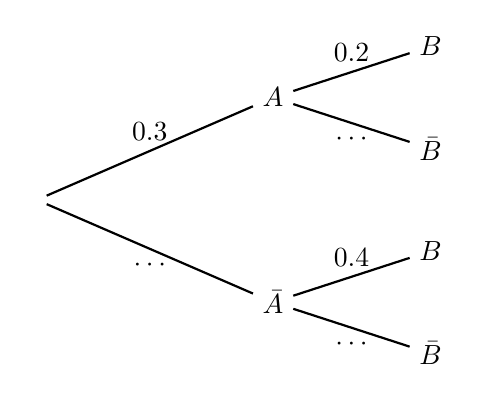
\begin{tikzpicture}[xscale=1,yscale=1]
			% Styles (MODIFIABLES)
			\tikzstyle{fleche}=[-,>=latex,thick]
			\tikzstyle{noeud}=[fill=white]
			\tikzstyle{feuille}=[fill=white]
			\tikzstyle{etiquette}=[midway,above]
			\tikzstyle{etiquette1}=[midway,below]
			% Dimensions (MODIFIABLES)
			\def\DistanceInterNiveaux{2}
			\def\DistanceInterFeuilles{1.3}
			% Dimensions calculées (NON MODIFIABLES)
			\def\NiveauA{(0)*\DistanceInterNiveaux}
			\def\NiveauB{(1.5)*\DistanceInterNiveaux}
			\def\NiveauC{(2.5)*\DistanceInterNiveaux}
			\def\InterFeuilles{(-1)*\DistanceInterFeuilles}
			% Noeuds (MODIFIABLES : Styles et Coefficients d'InterFeuilles)
			\node[noeud] (R) at ({\NiveauA},{(1.5)*\InterFeuilles}) {};
			\node[noeud] (Ra) at ({\NiveauB},{(0.5)*\InterFeuilles}) {$A$};
			\node[feuille] (Raa) at ({\NiveauC},{(0)*\InterFeuilles}) {$B$};
			\node[feuille] (Rab) at ({\NiveauC},{(1)*\InterFeuilles}) {$\bar{B}$};
			\node[noeud] (Rb) at ({\NiveauB},{(2.5)*\InterFeuilles}) {$\bar{A}$};
			\node[feuille] (Rba) at ({\NiveauC},{(2)*\InterFeuilles}) {$B$};
			\node[feuille] (Rbb) at ({\NiveauC},{(3)*\InterFeuilles}) {$\bar{B}$};
			% Arcs (MODIFIABLES : Styles)
			\draw[fleche] (R)--(Ra) node[etiquette] {$0.3$};
			\draw[fleche] (Ra)--(Raa) node[etiquette] {$0.2$};
			\draw[fleche] (Ra)--(Rab) node[etiquette1] {$\cdots$};
			\draw[fleche] (R)--(Rb) node[etiquette1] {$\cdots$};
			\draw[fleche] (Rb)--(Rba) node[etiquette] {$0.4$};
			\draw[fleche] (Rb)--(Rbb) node[etiquette1] {$\cdots$};
		\end{tikzpicture} 
	}
\end{exercise}

\begin{exercise} On dispose des informations suivantes d'une usine de production de jouets :
	\begin{enumerate}[leftmargin=*, label=\textbullet]
		\item Si le superviseur est de service, la probabilité qu'une pièce soit défectueuse   est de $2\%$.
		\item Si le superviseur n'est pas de service, la probabilité qu'une pièce soit défectueuse est de $3\%$.
		\item   Le superviseur est de service $39\%$ du temps.
	\end{enumerate}  
	On prend au hasard un nouveau jouet et on considère les événements suivants :\\
	$S$: \og le superviseur est de service \fg; \hspace*{5mm} $D$: \og le jouet est déféctueux\fg.
	\begin{enumerate}[leftmargin=*, label=\arabic*)]
		\item Traduire les données en termes de probabilités, en utilisant les événements $D$ et $S$.
		\item Représenter la situation par un arbre de probabilité.
		\item Quelle est la probabilité que la pièce soit déféctueuse ?
		\item Quelle est la probabilité que le superviseur soit de service sachant que la pièce est déféctueuse ?
	\end{enumerate}  
\end{exercise} 

\begin{exercise} 
	Une agence de voyage propose deux durées de séjours, le week-end ou la semaine, et deux types de destinations, France ou étranger.   Parmi les dossiers de l'agence on constate que: 
	\begin{enumerate}[leftmargin=*, label=\textbullet]
		\item  $60\%$ des séjours ont lieu en France;
		\item  $45\%$ des séjours en France durent une semaine;
		\item $75\%$ des séjours à l'étranger durent une semaine.
	\end{enumerate} 
	On choisit un dossier au hasard et on note:
	$F$ l’événement : \og Le séjour a lieu en France\fg et $S$ l'événement: \og Le séjour dure une semaine\fg.   
	\begin{enumerate}[leftmargin=*, label=\arabic*)]
		\item En utilisant les données de l'énoncé, précisez   $P\left(F\right)$;   $P_F\left(S\right)$ et $P_{\overline{F}}\left(S\right)$.
		\item Représenter la situation par un arbre de probabilité.
		\item Calculer $P_{\overline{F}}\left( \overline{S} \right)$, $P\left( F \cap \overline{S} \right)$ et  $P\left(S\right)$.
	\end{enumerate} 
\end{exercise}

\begin{exercise} 
	Dans l'ensemble des classes de terminale générale, en $2011$, il y avait $45\%$ de garçons. $88\%$ des filles ont été reçues au bac et seulement $86\%$ des garçons. On rencontre au hasard un élève qui était en terminale cette année-là. On note :
	\begin{enumerate}[label=\textbullet]
		\item $G$ l’événement : \og l'élève rencontré est un garçon \fg;
		\item $F$ l’événement : \og l'élève rencontré est une fille \fg;
		\item $R$ l’événement : \og l'élève rencontré a été reçu au bac \fg;
	\end{enumerate}
	\begin{enumerate}[leftmargin=*, label=\arabic*)]
		\item En utilisant les notations ci-dessus, traduire en langage des probabilités la phrase : \og $88\%$ des filles ont été reçues au bac\fg.
		\item Représenter la situation par un arbre de probabilité.
		\item Calculer les probabilités $P\left(G\cap R\right)$ et $P\left(F\cap R\right)$.
		\item En déduire $P\left(R\right)$.
	\end{enumerate}
\end{exercise}


\begin{exercise} 
	Une maladie affecte le cheptel bovin d'une région. On estime que $10\%$ des bovins sont atteints.
	
	Un test permet de diagnostiquer la maladie et on établit que :
	\begin{enumerate}[label=\textbullet,leftmargin=*]
		\item quand un animal est malade, le test est positif dans $85\%$ des cas;
		\item quand un animal n'est pas malade, le test est négatif dans $95\%$ des cas.
	\end{enumerate}
	Un animal est pris au hasard dans le cheptel bovin de cette région.
	\begin{enumerate}[leftmargin=*, label=\arabic*)]
		\item Représenter la situation par un arbre de probabilité.
		\item Déterminer la probabilité que le test soit erroné.
	\end{enumerate}
\end{exercise}

\begin{exercise} 
	On teste l'efficacité d'un médicament sur un échantillon d'individus  ayant un taux de glycémie anormalement élevé.
	
	\begin{enumerate}[label=\textbullet,leftmargin=*]
		\item Dans cette expérimentation, $50\%$ des individus prennent le médicament, les autres reçoivent un placébo. 
		\item On constate une baisse significative de ce taux chez $80\%$ des individus ayant pris le médicament.
		\item  On ne constate aucune baisse significative pour $90\%$ des individus ayant pris le placébo.
	\end{enumerate}
	On tire au hasard la fiche d'un participant à l'étude clinique. Calculer la probabilité que son taux de glycémie ait baissé significativement.
\end{exercise}


\begin{exercise} 
	A l'entrée d'un parc d'attraction, on peut acheter son billet soit à un guichet, soit à une caisse automatique.
	Dans les deux cas, on peut payer soit par carte bancaire, soit en argent liquide.
	
	$80\%$ des clients choisissent d'aller au guichet et utilisent alors leur carte bancaire dans $5\%$ des cas.
	
	Les utilisateurs de la caisse automatique paient par carte bancaire dans $65\%$ des cas.
	
	Chaque jour, on tire au hasard une des contremarques pour désigner l'heureux bénéficiaire du remboursement de son billet.
	
	Calculer la probabilité pour que le gagnant ait payé par carte bancaire.
\end{exercise}

\begin{exercise}
	Une entreprise vend des calculatrices. Le service après-vente s'est aperçu qu'elles pouvaient présenter deux types de défauts, l'un lié au clavier et l'autre lié à l'affichage.
	
	Des études statistiques ont permis à l'entreprise d'utiliser la modélisation suivante:
	\begin{enumerate}[label=\textbullet,leftmargin=*]
		\item La probabilité pour une calculatrice tirée au hasard de présenter un défaut de clavier est égale à $0,04$.
		\item En présence du défaut de clavier, la probabilité que la calculatrice soit en panne d'affichage est de $0,03$.
		\item En l'absence de défaut clavier, la probabilité de ne pas présenter de défaut d'affichage est de $0,94$.
	\end{enumerate} 
	On note $C$ l'événement \og la calculatrice présente un défaut de clavier \fg \hspace*{1mm} et $A$ l'événement \og la calculatrice présente un d\'efaut d'affichage \fg.
	\begin{enumerate}[leftmargin=*, label=\arabic*)]
		\item Déterminer les probabilités suivantes: $P_{\overline{C}}\left(\overline{A}\right)$, $P_C\left(A\right)$ et $P\left(C\right)$.
		\item Construire un arbre pondéré décrivant cette situation. 
		\item On choisit une calculatrice au hasard.
		\begin{enumerate}[leftmargin=*]
			\item Calculer la probabilité pour que la calculatrice présente les deux défauts.
			\item Calculer la probabilité pour que la calculatrice présente au-moins un défaut.
			\item Calculer la probabilité pour que la calculatrice présente le défaut d'affichage mais pas le défaut de clavier.
		\end{enumerate}
	\end{enumerate}	
\end{exercise}




\begin{exercise} 
	Pour recruter des stagiaires, une entreprise organise  des tests de sélection. Parmi les candidats qui se présentent aux épreuves, il y a $60\%$ de garçons. Après avoir pris connaissance des résultats aux tests, l'entreprise engage $70\%$ des garçons candidats et $80\%$ des filles candidates.
	
	On rencontre au hasard un candidat qui s'est présenté aux tests.
	\begin{enumerate}[leftmargin=*, label=\arabic*)]
		\item Quelle est la probabilité que ce candidat soit un garçon et qu'il soit engagé comme stagiaire?
		\item Quelle est la probabilité que ce candidat soit une fille et qu'elle soit engagée comme stagiaire?
		\item Calculer la probabilité que ce candidat soit engagé.
	\end{enumerate}
\end{exercise}

\begin{exercise} 
	Une situation est modélisée par l'arbre ci-dessous. $A$ et $B$ désignant deux événements. En utilisant l'arbre de gauche, compléter l'arbre de droite:\\
	\parbox{0.5\linewidth}{ 
		% Racine à Gauche, développement vers la droite
		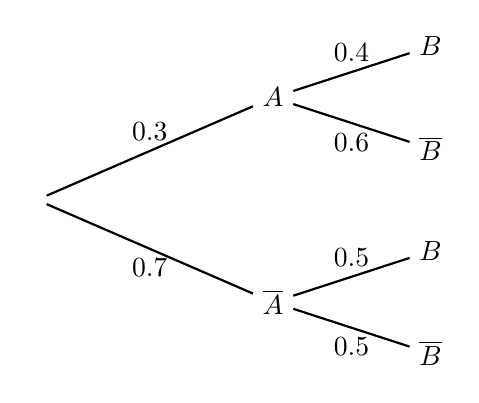
\begin{tikzpicture}[xscale=1,yscale=1]
			% Styles (MODIFIABLES)
			\tikzstyle{fleche}=[-,>=latex,thick]
			\tikzstyle{noeud}=[fill=white]
			\tikzstyle{feuille}=[fill=white]
			\tikzstyle{etiquette}=[midway,above]
			\tikzstyle{etiquette1}=[midway,below]
			% Dimensions (MODIFIABLES)
			\def\DistanceInterNiveaux{2}
			\def\DistanceInterFeuilles{1.3}
			% Dimensions calculées (NON MODIFIABLES)
			\def\NiveauA{(0)*\DistanceInterNiveaux}
			\def\NiveauB{(1.5)*\DistanceInterNiveaux}
			\def\NiveauC{(2.5)*\DistanceInterNiveaux}
			\def\InterFeuilles{(-1)*\DistanceInterFeuilles}
			% Noeuds (MODIFIABLES : Styles et Coefficients d'InterFeuilles)
			\node[noeud] (R) at ({\NiveauA},{(1.5)*\InterFeuilles}) {};
			\node[noeud] (Ra) at ({\NiveauB},{(0.5)*\InterFeuilles}) {$A$};
			\node[feuille] (Raa) at ({\NiveauC},{(0)*\InterFeuilles}) {$B$};
			\node[feuille] (Rab) at ({\NiveauC},{(1)*\InterFeuilles}) {$\overline{B}$};
			\node[noeud] (Rb) at ({\NiveauB},{(2.5)*\InterFeuilles}) {$\overline{A}$};
			\node[feuille] (Rba) at ({\NiveauC},{(2)*\InterFeuilles}) {$B$};
			\node[feuille] (Rbb) at ({\NiveauC},{(3)*\InterFeuilles}) {$\overline{B}$};
			% Arcs (MODIFIABLES : Styles)
			\draw[fleche] (R)--(Ra) node[etiquette] {$0.3$};
			\draw[fleche] (Ra)--(Raa) node[etiquette] {$0.4$};
			\draw[fleche] (Ra)--(Rab) node[etiquette1] {$0.6$};
			\draw[fleche] (R)--(Rb) node[etiquette1] {$0.7$};
			\draw[fleche] (Rb)--(Rba) node[etiquette] {$0.5$};
			\draw[fleche] (Rb)--(Rbb) node[etiquette1] {$0.5$};
		\end{tikzpicture}
	}
	\hfill
	\parbox{0.5\linewidth}{  
		% Racine à Gauche, développement vers la droite
		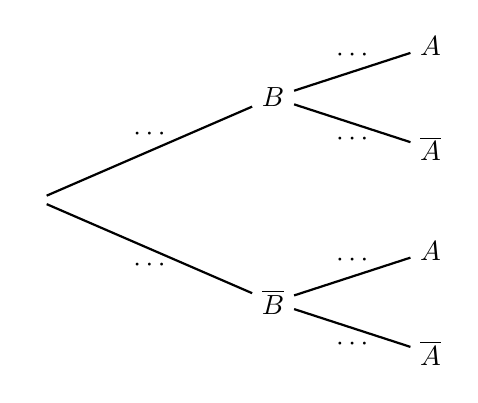
\begin{tikzpicture}[xscale=1,yscale=1]
			% Styles (MODIFIABLES)
			\tikzstyle{fleche}=[-,>=latex,thick]
			\tikzstyle{noeud}=[fill=white]
			\tikzstyle{feuille}=[fill=white]
			\tikzstyle{etiquette}=[midway,above]
			\tikzstyle{etiquette1}=[midway,below]
			% Dimensions (MODIFIABLES)
			\def\DistanceInterNiveaux{2}
			\def\DistanceInterFeuilles{1.3}
			% Dimensions calculées (NON MODIFIABLES)
			\def\NiveauA{(0)*\DistanceInterNiveaux}
			\def\NiveauB{(1.5)*\DistanceInterNiveaux}
			\def\NiveauC{(2.5)*\DistanceInterNiveaux}
			\def\InterFeuilles{(-1)*\DistanceInterFeuilles}
			% Noeuds (MODIFIABLES : Styles et Coefficients d'InterFeuilles)
			\node[noeud] (R) at ({\NiveauA},{(1.5)*\InterFeuilles}) {};
			\node[noeud] (Ra) at ({\NiveauB},{(0.5)*\InterFeuilles}) {$B$};
			\node[feuille] (Raa) at ({\NiveauC},{(0)*\InterFeuilles}) {$A$};
			\node[feuille] (Rab) at ({\NiveauC},{(1)*\InterFeuilles}) {$\overline{A}$};
			\node[noeud] (Rb) at ({\NiveauB},{(2.5)*\InterFeuilles}) {$\overline{B}$};
			\node[feuille] (Rba) at ({\NiveauC},{(2)*\InterFeuilles}) {$A$};
			\node[feuille] (Rbb) at ({\NiveauC},{(3)*\InterFeuilles}) {$\overline{A}$};
			% Arcs (MODIFIABLES : Styles)
			\draw[fleche] (R)--(Ra) node[etiquette] {$\cdots$};
			\draw[fleche] (Ra)--(Raa) node[etiquette] {$\cdots$};
			\draw[fleche] (Ra)--(Rab) node[etiquette1] {$\cdots$};
			\draw[fleche] (R)--(Rb) node[etiquette1] {$\cdots$};
			\draw[fleche] (Rb)--(Rba) node[etiquette] {$\cdots$};
			\draw[fleche] (Rb)--(Rbb) node[etiquette1] {$\cdots$};
		\end{tikzpicture}
	}
\end{exercise} 
\begin{exercise} 
	On considère deux événements $A$ et $B$ tels que $P(A)=p$, $P(B)=P(\overline{A})$ et $P(A \cap B)=0,2p+0,15$.
	\begin{enumerate}
		\item Montrer que, pour tout $p \in \mathbb{R}$, $-p^2+0,8p-0,15=(0,3-p)(p-0,5)$
		\item Trouver la probabilité $p$ telle que $A$ et $B$ soient indépendants.
	\end{enumerate}
\end{exercise} 
\begin{exercise} 
	On considère deux événements $A$ et $B$ tels que $P(A \cap B)=0,8$ et $P(A \cup B)=0,9$.
	\begin{enumerate}
		\item Montrer que, pour tout $p \in \mathbb{R}$, $x^2-1,7x+0,8=(x-0,85)^2+0,0775$.
		\item Montre que $A$ et $B$ ne peuvent pas être indépendants.
	\end{enumerate}
\end{exercise} 
%----------------------------------------------------------------------------------------
%	 
%----------------------------------------------------------------------------------------
\end{document}
